\documentclass[conference]{IEEEtran}

%% Custom TeX

%% 
%% Notes on notational conventions:
%% -> is used for logical implication, \rightarrow
%% => is used for meta implication, \implies
%% We use . in \exists and \forall in ETL
%% We use , and there exists and for all in meta logic
%%

\usepackage{srcltx}
\usepackage{url}
\usepackage{latexsym,amsmath,amssymb,stmaryrd}
\usepackage[standard]{ntheorem}

\renewcommand{\bfdefault}{b}

\usepackage{xspace}
\usepackage{enumerate}
%\usepackage[pdftex,hyperref,svgnames]{xcolor}
\usepackage{graphics}
\usepackage{listings}
\usepackage{supertabular}
\usepackage{stackrel}
\usepackage{marvosym}
\usepackage{pgf,tikz}
\usepackage{mdframed}
\usepackage{mathpartir}
\usepackage{etoolbox}
\usepackage{color,soul} % Highlighting

% Listings
\newcommand{\code}[1]{\text{\lstinline!#1!}}

\definecolor{lightgreen}{rgb}{.85,.95,.85}
\definecolor{lightblue}{rgb}{.85,.90,1}
\definecolor{lightred}{rgb}{.95,.85,.85}
\definecolor{lightgrey}{rgb}{.95,.95,.95}
\sethlcolor{lightred}

\definecolor{drkyellow}{rgb}{0.4,0.3,0}
\definecolor{drkred}{rgb}{0.5,0,0}
\definecolor{drkgreen}{rgb}{0,0.5,0}

\definecolor{dkgreen}{rgb}{0.1,0.40,0.1}

\definecolor{dkred}{rgb}{0.5,0,0}
\definecolor{medred}{rgb}{0.6,0,0}
\definecolor{gray}{rgb}{0.5,0.5,0.5}
\definecolor{mauve}{rgb}{0.58,0,0.82}

\newcommand{\myparagraph}[1]{\paragraph{#1.}}

\newcommand{\lstrule}{%
 \hspace{1mm}%
 \color{gray}{\rule[1.18mm]{0.8\textwidth}{0.1pt}}%
 \hspace{\fill}%
}

%% TODO: Make the listings look prettier

\lstset{ %
  language=caml,                    % the language of the code
  morecomment=[l]{--},          % add Haskell comment style
  basewidth=0.5em,
  lineskip={-2.35pt},
%  aboveskip=5mm,
%  belowskip=-5mm,
  columns=fixed,
  basicstyle=\small\ttfamily,
%  identifierstyle=\textbf,
%  keywordsprefix=\#,
  literate={->}{$\rightarrow$}2
           {=>}{$\Rightarrow$}2
           {<-}{$\leftarrow$}2
           {..}{$\cdots$}2
           {fun}{$\lambda$}1
           {||}{$\parallel$}1
           {**}{$\times$}2,
  escapechar=@,
  escapeinside={/**}{*/},
  numbers=left,                   % where to put the line-numbers
  numberstyle=\tiny\color{gray},  % the style that is used for the line-numbers
  stepnumber=1,                   % the step between two line-numbers. If it's 1, each line 
                                  % will be numbered
  numbersep=5pt,                  % how far the line-numbers are from the code
  showspaces=false,               % show spaces adding particular underscores
  showstringspaces=false,         % underline spaces within strings
  numberblanklines=false,
  showtabs=false,                 % show tabs within strings adding particular underscores
%  frame=single,                   % adds a frame around the code
%  frame=lines,
  rulecolor=\color{gray},        % if not set, the frame-color may be changed on line-breaks within not-black text (e.g. commens (green here))
  tabsize=2,                      % sets default tabsize to 2 spaces
%  captionpos=b,                   % sets the caption-position to bottom
  breaklines=false,                % sets automatic line breaking
  breakatwhitespace=false,        % sets if automatic breaks should only happen at whitespace
%  title=\lstname,                   % show the filename of files included with \lstinputlisting;
%  keywordstyle=\color{blue},          % keyword style
%  identifierstyle=\color{drkgreen},     
%  backgroundcolor=\color{lightgrey},
  commentstyle=\color{dkred}\itshape,       % comment style
  stringstyle=\color{mauve}         % string literal style
}

\lstset{emph={},emphstyle={}}%
\lstset{morekeywords={\!, (, \), \., \<, \>, ref, in, if,then,else,let, install, <,>},keywordstyle={\color{blue}\bfseries}}%

%% Theorem stuff
\theoremstyle{definition}
\newtheorem{defn}{Definition}[section]
\newtheorem{lem}{Lemma}[section]
\newtheorem{thm}{Theorem}[section]

\newcommand{\aset}[1]{\{#1\}}
\newcommand{\dom}{\mathop\textit{dom}\nolimits}

%% Names of things
\newcommand{\tvetl}{TVETL\xspace}

\newcommand{\sfmt}[1]{\textsf{#1}}
\newcommand{\sch}{\textit{ch}}
\newcommand{\prin}{\textit{O}}
\newcommand{\loc}{\ell}
\newcommand{\sassign}[2]{#1 := #2}
\newcommand{\scase}[2]{\sfmt{case}~#1~\sfmt{of}~#2}
\newcommand{\sderef}[1]{!#1}
\newcommand{\sfalse}{\sfmt{false}}
\newcommand{\sif}[3]{\sfmt{if}~#1~\sfmt{then}~#2~\sfmt{else}~#3}
\newcommand{\sinl}{\sfmt{inl}}
\newcommand{\sinr}{\sfmt{inr}}
\newcommand{\sinstall}[2]{\sfmt{install}~#1~#2}
\newcommand{\sdeclassify}[1]{\sfmt{declassify}~#1}
\newcommand{\sref}[1]{\sfmt{ref}~#1}
\newcommand{\denot}[1]{\ensuremath{\llbracket #1 \rrbacket}}
\newcommand{\ssend}[2]{\sfmt{send}~#1~#2}
\newcommand{\strue}{\sfmt{true}}
\newcommand{\sunit}{\sfmt{unit}}
\newcommand{\sreduce}{\Downarrow}
\newcommand{\treduce}{\rightarrow}
\newcommand{\partialfun}{\rightharpoonup}
\newcommand{\ltrue}{\ensuremath{\top}}
\newcommand{\lfalse}{\ensuremath{\bot}}
\newcommand{\config}[1]{\langle{}#1\rangle{}}
\newcommand{\program}[1]{\ensuremath{\mathcal{#1}}}
\newcommand{\restr}[2]{\ensuremath{\left.#1\right|_{#2}}}
\newcommand{\modelsrcon}{\models^{r}}
\newcommand{\amodels}{\models^{A}}
\newcommand{\judge}{\vdash}
\newcommand{\xv}{p}
\newcommand{\filter}{\upharpoonright}
\newcommand{\restrict}{\upharpoonright}
\newcommand{\etlb}{ETLB\xspace}
\newcommand{\hyperltltwo}{HyperLTL\xspace}

\newcommand{\absstate}{\Sigma^s}
\newcommand{\tvar}{x^t}

\newcommand{\traces}[1]{\mathcal{T}(#1)}
\newcommand{\tick}[1]{#1^{+}}
\newcommand{\atom}{A}

\newcommand{\tr}{t\xspace}
\newcommand{\typ}{\tau}
\newcommand{\tint}{\textit{int}}
\newcommand{\tset}{\ensuremath{\mathcal{T}}\xspace}
\newcommand{\tsets}{\ensuremath{\mathcal{T}^s}\xspace}
\newcommand{\pset}{\ensuremath{\mathcal{P}}}
\newcommand{\tnext}{\mathcal{X}}
\newcommand{\talways}{\mathcal{G}}
%\newcommand{\tfuture}{~\mathcal{F}~}
\newcommand{\tevent}{\lozenge}
\newcommand{\tfuture}{\mathcal{F}}
\newcommand{\tuntil}{~\mathcal{U}~}
\newcommand{\tsince}{~\mathcal{S}~}
\newcommand{\tpast}{~\mathcal{P}~}
\newcommand{\tknows}[1]{\mathcal{K}_{#1}}
\newcommand{\tatmost}[1]{\mathcal{N}_{#1}}
\newcommand{\tpossible}[1]{\mathcal{L}_{#1}}
\newcommand{\tthen}{~\textit{then}~}
\newcommand{\tlast}[2]{\textit{last}(#1, #2)}
\newcommand{\limplies}{\rightarrow}
%\newcommand{\tforall}{\hbox{forall}~}
\newcommand{\texists}{\hbox{exists}~}
\newcommand{\tcurrent}[1]{\hbox{current}_{#1}~}
\newcommand{\tval}[1]{\textit{value}(#1)}
\newcommand{\trelease}{\rhd}
\newcommand{\evt}{\eta}
\newcommand{\mimplies}{\Rightarrow}
\newcommand{\with}{\&}

%% for comments
\newcommand{\comment}[3][\color{red}]{{#1{[{#2}: {#3}]}}}
\newcommand{\kris}[1]{\comment[\color{orange}]{kris}{#1}}
\newcommand{\jeff}[1]{\comment[\color{green}]{JSF}{#1}}
\newcommand{\mrc}[1]{\comment[\color{blue}]{MRC}{#1}}
\newcommand{\thickhline}{\noalign{\hrule height 1pt}}
\newcommand{\low}{\text{L}\xspace}
\newcommand{\high}{\text{L}\xspace}

\newcommand{\lang}{revea$\lambda$\xspace}

%% End of custom TeX

%\conferenceinfo{XXX} {XXX}
%\CopyrightYear{XXX}
%\copyrightdata{XXX}

%\pagenumbering{arabic}

\begin{document}

\pagestyle{plain}

\title{Information Flow Policies for User Interaction}
\maketitle

\begin{abstract}
  Researchers have explored a wide range of declassification policies
  in the context of \emph{batch} programs --- those that produce an
  output given an input. In this paper, we explore declassification in
  the context of \emph{interactive, GUI-based} software, such as
  mobile apps. We observe that in many apps, declassification is
  controlled by the user via the GUI, and may change over time as an
  app executes. We introduce revea$\lambda$, a core language that can
  model interactive GUI apps including user interactions, time varying
  input, and declassification. In revea$\lambda$, we use an epistemic
  temporal logic to specify security policies; the logic is powerful
  enough to capture notions of interactive declassification we have
  seen in a range of apps that deal with time varying secret input. We
  prove that many standard security and declassification properties
  have counterparts in our logic, including a set of new polices that
  cannot be expressed in prior work.  We also show how to use symbolic
  execution to check these policies, presenting a concrete
  counterexample (in the form of a user input sequence along with a
  set of secret inputs) when one exists.  We implement our symbolic
  execution semantics in a symbolic executor for Android and apply it
  to a range of example apps.
\end{abstract}

% This leads developers to adding a number of potentially unsound and
% awkward declassification measures to languages which cannot cleanly
% express declassification information.

\section{Introduction}
\label{sec:introduction}

Applications that manipulate our private data are now ubiquitous: web
services access our interests and contacts to serve targeted ads, apps
use our location to provide context aware computing, and sensitive
data often quickly leaks in subtle and unintended ways as a
consequence of providing an enhanced user experience.  Understanding
precisely how we can define and enforce security policies for
privilaged data has been the subject of language based security since
it's inception.  And yet, adapting existing techniques to modern
applications has proven problematic for a variety of reasons.
\kris{elaborate? Cite?} In this paper we provide a core formalism for
interactive apps that manipulate dynamic (time-varying) data and communicate
with external principals, inspired by Android app semantics.  We
present a new logic that allows us to to constrain what an observer
may learn about data based on release policies that relate user input
to released information.  We show that this logic can express standard
information flow policies and is uniquely suited for stating new
policies that speak about release of dynamic secrets.
Finally, we implement our logic in a symbolic executor for Android
programs, which certifies that our example applications meet their
specifications.

Current applications written for Android and iOS use access control
mechanisms (enforced by the platform) to constrain secret data, such
as the list of contacts or fine grained location information.  This
technique allows users to be confident that some data is not leaked to
an app, but is insufficient if an app legitimately needs to compute
with the data.  In these situations, the users are either forced to
trust that their information is used correctly, or not install the
app.  However we observe that secret data is frequently guarded by
some user input (such as an explicit GUI control that allows fine
grained location to be released).  Our logic allows us to express
policies that relate these user inputs to information that can be
released by the app, allowing the app to leak only the portion of the
information that is explicitly specified.

We present a new logic based on Epistemic Temporal Logic
\cite{Balliu:11} that serves as an extensional specification of the
security properties of apps in our formalism. We show how it can be
used to specify properties for a variety of example programs.  ETL
allows us to use temporal modalities to speak about when events (such
as release conditions) happen in the program, and also what observers
learn as they watch evolving computation via communication channels.
This allows us to state policies such as ``the observer does not learn
the value of the secret before the button is pressed.''  We extend
previous work on epistemic temporal logic to deal with traces
generated by our semantics, allowing us to speak about programs that
manipulate dynamic inputs and communicate with an external
observer (such as a web service).  To prove the utility of our logic,
we show how a variety of standard security policies (such as
noninterference and gradual release) have equivalent analogues in ETL.

Specifically, we show that ETL can encode gradual release for dynamic
secrets.  This allows us to express (and subsequently check) the
policies for the example programs shown in Section~\ref{sec:examples}.
Figure~\ref{fig:ni-implication} shows the properties and equivalences
we present in section~\ref{sec:etl}, with arrows indicating
subsumption of properties (e.g., noninterference implies dynamic
noninterference).  Specifically, they are:

\begin{description}
\item[Noninterference] \hfill \\
  A program satisfies noninterference if an observer learns nothing
  about the initial secret input by observing the execution of the
  program.  We lift this to a trace based setting and state a formula
  in ETL that is equivalent to the traditional definition of
  noninterference given in \kris{cite}.
\item[Gradual release] \hfill \\
  Gradual release is a mechanism by which release of static input
  secrets can be controlled by stating precisely what information is
  released at various points in the program.  We show that ETL can be
  used to state gradual release for static input secrets using LTL
  formulas for release events and formulas that use knowledge
  modalities to constrain upper bounds on knowledge.
\item[Dynamic noninterference] \hfill \\
  Programs may read secret data that varies over time via inputs such
  as location, sensors, or passwords.  We state an analogue of
  noninterference for dynamically changing secrets in ETL and show how
  it is equivalent to the definition given in \cite{O'Neill:06}
  \kris{wrong cite I think we want 08}.
\item[Dynamic gradual release] \hfill \\
  Is a property that allows dynamic secrets to be declassified
  based on some event in the program, essentially combining dynamic
  input and gradual release.  In section~\ref{sec:examples} we show
  how this is a natural way to express rich security properties via a
  set of examples and show how it implies the other properties.
\end{description}

\begin{figure}
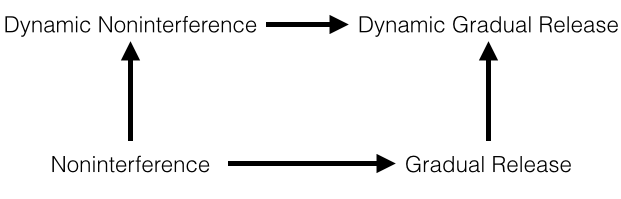
\includegraphics[width=\linewidth]{ni-implication}
\caption{Relationship among release policies.}
\label{fig:ni-implication}
\end{figure}

% The paper proceeds as follows: we first present a set of motivating
% examples in section~\ref{sec:examples}.  These examples include
% programs in our formalism and policies written in our logic.
% Section~\ref{sec:formalism} presents a core operational semantics for
% reactive programs that manipulate secret data.  Section~\ref{sec:etl}
% then presents our logic based on the operational semantics, proving
% that we can encode useful release policies using the logical
% primitives.  Section~\ref{sec:symbolic} then shows how we implement
% the example applications and policies in our symbolic executor,
% detailing how we assemble proof obligations that are discharged by a
% solver based on an exploration of the input
% space. Section~\ref{sec:related-work} compares our work against
% related work.  Finally, we comment on future work in
% section~\ref{sec:future} and conclude in section \ref{sec:conclusion}.

\section{Examples}
\label{sec:examples}

\jeff{I don't really like the font that the apps are written in. I
  tried changing it but couldn't get that to work. Why not use
  flexible columns, sans serif font?}

We begin our presentation with examples illustrating a range of apps
along with the formulas in our logic that demonstrate their security
policies. We write our apps in an OCaml-like language, similar to our
formal model in Section~\ref{sec:formalism}, and their structure mimic
the structure of Android apps: Each app has an \code{onCreate}
function that is called when the app starts. That function is
responsible for creating GUI elements with corresponding callbacks,
which carry out the appropriate actions upon button clicks, checkbox
selects, etc. Apps can also send data over the network. We will
explain our language and release policy notation in more detail as we
go through the examples.

\subsection{Noninterference}

One popular program property considered in the literature is
noninterference, meaning that the observer learns nothing about the
secret input to the program by observing its output.  While this can
be implemented using access control, many apps use secret data in safe
ways, but do not leak the information to the observer. As an example,
consider the following application that allows the user to browse
their contacts and send a checkbox's value to the server:

\begin{lstlisting}[name=Ex]
let handle_s s =
  send id_t s

let handle_c v =
  if (v == true)
    send netout 1
  else 
    send netout 0

let onCreate (contacts) = 
  new_textbox id_t;
  new_checkbox id_c "Switch on?"; /** \label{line:switch} */
  install id_c handle_c;
  new_spinner id_s contacts "Contacts"; /** \label{line:selectspinner} */
  install id_s handle_s
\end{lstlisting}

Upon initialization, the \code{onCreate} function runs.  This creates
a textbox, and installs two handlers: one to handle the checkbox
toggle (line~\ref{line:switch}), another to handle the contact
selection (line~\ref{line:selectspinner}).  When the checkbox is
toggled, its new value is passed to the handler \code{handle_c}, where
its value is subsequently sent to the network by sending it to the
\code{netout} channel.  When the user selects a value from the
spinner, it is written to the textbox: but nothing about the contacts
is ever released to the network.

In our logic, we write down the following formula that corresponds to
noninterference:

\begin{displaymath}
  \begin{array}{c}
    \talways \Big( \forall x. \tpossible{\prin}(\code{contacts} = x)
    \Big )
  \end{array}
\end{displaymath}

The observer reads the writes from the \code{netout} channel.  In our
logic, $\tpossible{\prin}(contacts = x)$ means that --- from the
observer's point of view --- it must always be \emph{possible} that
\code{contacts} is equal to $x$, for any value of $x$.  In other words,
the observer cannot rule out any value $x$ for the value of
\code{contacts}.  The $\prin$ subscript on the $\tpossible{}$ modality
is a set of channels that the observer can read.  In this paper, we
always use the \code{netin} and \code{netout} channels.

\subsection{Releasing static secrets}

\kris{some intro text here...?}

\paragraph*{Noninterference until a condition} 

As another example, consider an app that shares various pieces of
information depending on the settings of various checkboxes:

\begin{lstlisting}[name=Ex]
let email_release = ref false
let phone_release = ref false

let handle_b =
  if !email_release && !phone_release then
    send netout (email ^ "|" ^ phone)
  else if !email_release
    send netout email
  else if !phone_release
    send netout phone

let handle_c r v =
  r := v
    
let onCreate () = 
  new_checkbox id_e "Email?";
  install id_e (handle_c email_release);
  new_checkbox id_ph "Phone #?";
  install id_ph (handle_c phone_release);
  new_button id_b "Send";
  install id_b handle_b
\end{lstlisting}

This app first creates two checkboxes using the \code{new_checkbox}
functions.  When the user provides inputs to these checkboxes, their
values (either \code{true} or \code{false}, indicating presence or
lack of a check) will be written on channels \code{id_e} and
\code{id_ph} respectively.  To read values on these channels, the app
installs handlers that receive values on these channels.  The app
provides the handler \code{handle_c email_release} for the \code{id_e}
channel.  Note that here we use currying, \code{handle_c r} evaluates
to a function that takes an argument \code{v} and sets the value of r
to \code{v}.  This means that, whenever the user toggles the email
checkbox, the value is sent on the \code{id_e}, and then the handler
sets \code{email_release} to \code{true} if it was checked, and
\code{false} otherwise.

The app then creates a button and installes a handler for its presses
on the \code{id_b} channel.  The handler, \code{handle_b}, checks the
values of the \code{email_release} and \code{phone_release}
references, and sends the values of \code{email} and \code{phone}
(assumed to be secret) to the network based on the settings.

We can define the policy as follows:

\begin{displaymath}
  \begin{array}{lcc}
    \forall x. & \talways & \big( \lnot (Declass_e) \rightarrow
    \tpossible{\prin} (x = \code{email}) \big) \\
    & \land & \big( \lnot (Declass_p) \rightarrow 
    \tpossible{\prin} (x = \code{phone}) \big)
  \end{array}
\end{displaymath}  

The formula can be read as follows: at any point in time, if the user
has not declassified the email (an LTL predicate we define below), then
the observer should believe that the email could be any value $x$.

We define the predicate $Declass_e$ as a formula in LTL (linear
temporal logic), a temporal logic that allows us to speak about
ordering of events in time.  Our logic includes LTL as a subsuet, and
LTL allows to formally specify conditions
under which inforamtion can be declassified as a series of interactions
the user takes with the GUI.  We can define $Declass_e$ as follows:

\begin{displaymath}
  \begin{array}{c}
    Declass_e =  \lnot \code{id\_e?*@*} \tsince \big(
    \code{id\_e?true@*} \tfuture (\code{id\_b?()@*}) \big)
  \end{array}
\end{displaymath}  

Our system consists of timestamped read and write events on channels.
We use the logical notation \code{id_e?v@i} to denote that a read
event occured on channel \code{id_e} that carried the value \code{v}
at timestamp \code{i}, but allow the value and timestamp to be
wildcards.  This formula uses the $\tsince$ modality to say that
\emph{since} the email checkbox became true (\code{id\_e?true@*}) --
there was eventually a button press $\tfuture (\code{id\_b?()@*})$ and
there were no values written to the \code{id_e} channel.  This rules
out the case where the user checked the box, then unchecked it, then
pressed the button: in which case the information should not be
declassified. We define a similar policy for $Declass_p$.

We use the following syntactic sugar to encode the policy more simply:

\begin{displaymath}
  \begin{array}{c}
    last(\code{id\_e}) = \code{true} , \code{id_b} = () \rhd email \\
    last(\code{id\_p}) = \code{true} , \code{id_b} = () \rhd phone \\
  \end{array}
\end{displaymath}

Which means that the \code{email} is declassified whenever the button
has been pressed, and the last value of the \code{id_e} channel was
true, and similar for the phone number.

\paragraph*{Sharing a designated contact}
\label{example:contacts}

Consider an app that sends a contact selected by the user to a remote
party:

\begin{lstlisting}[name=Ex]
let cur_contact = ref None

let handle_s s =
  current_contact := Some s

let handle_b () =
  case (!cur_contact) of
    | None -> ()
    | Some s -> send netout s

let onCreate = 
  new_button id_b "Send contact"; /** \label{line:button} */
  install id_b handle_b;
  new_spinner id_s contacts "Contacts"; /** \label{line:spinner} */
  install id_s handle_s
\end{lstlisting}

Here the \code{onCreate} function creates two GUI elements, a button
(line~\ref{line:button}) and a spinner allowing the user to select one
from the set of all contacts, which is assumed to be secret
(line~\ref{line:spinner}).  Each GUI element is associated with a
\emph{channel}---\code{id_b} for the button and \code{id_s} for the
spinner. The framework sends messages on these channels whenever the
corresponding GUI element is used.  Note that the channels are free
variables of the app so we can use them in our security policies.

After creating the button and spinner, the app uses \code{install} to
register callbacks to receive messages on the appropriate
channels. Now \code{onCreate} exists, and the app waits for its
callbacks to be invokes. When the spinner selection is changed, the
\code{handle_s} function is called, which stores the selected contact
in a global variable. When the button is clicked, \code{handle_b}
retrieves the last-selected contact (if any) and sends it over the
network, on the \code{netout} channel.

The policy that we wish to enforce is that the observer (reading from
the \code{netout}) only learns values
from the contacts that was last selected when the button was pressed.
For example, suppose that the contact list is $[\text{Alice},
\text{Bob}, \text{Charlie}]$.  Consider the following sequence of
events:

\begin{displaymath}
  \begin{array}{c}
    \code{id\_s(Alice)}, \code{id\_s(Charlie)}, \code{id\_b},
    \code{id\_s(Bob)}, \code{id\_b}
  \end{array}
\end{displaymath}

We wish to say that our policy is that when \code{id\_b} (the button)
is clicked, the observer can learn that Charlie is a member of the
contacts list, but that at that point, the observer still cannot know
whether or not Alice (or Bob) is a contact.  Similarly, once
\code{id\_b} is clicked the second time, the observer can learn that
Charlie and Bob are contacts (since knowledge grows monotonically over
time).  In our logic, we express this formula:

\begin{displaymath}
  \begin{array}{c}
    \forall x. \talways \big( \lnot (Declass~x) \rightarrow \tpossible{\prin} (x \in contacts) \big)
  \end{array}
\end{displaymath}
which means, ``for any contact $x$, if the contact $x$ has not yet
been declassified, the observer must not know whether or not $x$ is in the
set $contacts$.''

We define whether a contact has been declassified based on an LTL formula:

\begin{displaymath}
  \begin{array}{c}
    Declass~x =  \lnot \code{id\_s?*@*} \tsince \big(
    \code{id\_s?x@*} \land \tfuture (\code{id\_b?()@*}) \big)
  \end{array}
\end{displaymath}

Which can be read, ``since the last time that the button was pressed,
whence the most recent value of the spinner was $c$, there have been
no selected values on the spinner channel.''

This policy is a form of gradual release \cite{Askarov:2007}: the
observer's knowledge about an initial secret grows over time at
specific designated release points.  Using our logic, we can
explicitly relate the information that is released to the action the
user took using these release predicates.

% In section~\ref{sec:etl}, we show how to systematically write policies
% of this form in our logic using the epistemic modalities and LTL
% release predicates, and in section~\ref{sec:symbolic} we show how we
% use symbolic execution to enforce policies of this type.

\subsection{Dynamic Noninterference}

Our logic can also handle policies for data that changes over time.

\subsection{Communicating with the observer}

While applications can send messages to the observer, the observer can
also influence execution in the application by sending messages to the
application.  The next application allows the observer to query the
user's location, but the user can also choose between allowing
location and disallowing access.  Unless the user has explicitly
allowed the location to be disclosed, the program does not send a
response:

\begin{lstlisting}[name=Ex]
let last_location = ref None
let allowed = ref false

let handle_net _ =
  case (!last_location) of
    | None -> ;
    | Some loc -> send netout loc

let handle_loc l =
  if (!allowed) then
    last_location := Some l
  else
    last_location := None

let handle_c v =
  allowed := v

let onCreate () = 
  new_checkbox id_c "Query location?";
  install id_c handle_c;
  install loc handle_loc;
  install netin handle_net;
\end{lstlisting}

\begin{displaymath}
  \begin{array}{lcc}
    \forall v. & \talways & \big( \lnot (Released_e) \rightarrow \lnot
    \tpossible{\prin} (v = \code{email}) \big)
  \end{array}
\end{displaymath}  

\jeff{Say, where Released\_e is defined as above}

\jeff{You haven't really explained here why this is an interesting
  policy---it looks pretty much exactly the same as the previous
  policy, from section B. Maybe that means the policy isn't quite
  right? It seems like you could add that no information is released
  until there's a read from the netin channel. Also, why is the L
  negated here?}


\paragraph*{Toggling resolution of collected data}

Next we consider an app that allows the user's location to be sent to

Along with releasing static data such as contacts and email addresses,
many applications interact with and release dynamic data sources,
such as such as location information.  The user may feel uncomfortable
revealing their fine grained information to the application at any
time, but may be okay revealing their location when they allow it:
e.g., when they check a box.  Because of this, the app might present a
configuration option to the user that allows them to toggle the data
collection between fine grained and coarse grained information.  As an
example, a restaurant recommendation might have options that give ads
to the user based on their city, but might also recommend restaurants
in their neighborhood.

One example implementation might use a checkbox to select whether the
app should be sharing fine grained information, and collect fine
grained information only at times when the checkbox is checked:

\begin{lstlisting}[name=Ex]
type prec = Truncate | Full
let prec_policy = ref Truncate

let handle_r v =
  if v = 0 then
    prec_policy := Truncate
  else if v = 1 then
    prec_policy := Full

let handle_loc loc = 
  case !prec_policy of
    Truncate -> send netout (truncate loc)
  | Full -> send netout (loc)
  
let onCreate () = 
  new_radio_buttons id_r
    [(0, "Truncate"); (1, "Full precision")];
  install id_r handle_r;
  install loc handle_loc
\end{lstlisting}

Here, \code{loc} is a dynamic source. \jeff{Need to explain what
  this means---write ``time varying'' in italics to indicate you're
  defining it, and then say in other words what you mean---that the
  location changes depending on when its retrieved.}
In our semantics,
installing a handler on the location source \code{loc} will
nondeterministically input the location, modeling the nondeterministic
location handler callback found in Android and other systems.
\jeff{It's unclear what nondeterministically means here. I think what
  happens is, the framework will periodically call handle\_loc, at
  some interval, to update the location. From the app's perspective,
  this is nondeterministic, because a new location might come in at
  any time.}
Our
semantics uses a message queue to serially order events that happen in
the system, which guarantees that when the location callback handler
(\code{handle\_loc}) runs, the policy has been correctly set by the
code. \jeff{I don't understand the previous sentence. You can't write
  text like this that assumes the reader understands the figure
  without your help---you need to walk the reader through the
  figure. By this time, the reader understands how this GUI stuff
  works, so you don't need to do it in a huge amount of detail. But
  you do need to say, installs radio button, if this is clicked then
  that happens, etc. Another way to put it: Imagine you were sitting
  next to someone and working through the paper with them. You
  wouldn't show them this code and say what you just wrote. You'd
  first explain how the code works, and then give the high-level take away.}

We can write a policy which uses the current value of the checkbox to
dictate an upper bound on the current location information: \jeff{In
  what sense is this an upper bound? I think there's no
  overapproximation going on here, which is what your previous
  sentence implied. It's just a precise description of the information
  that's released.}

\begin{displaymath}
  \begin{array}{l}
    \talways Fine \rightarrow \Big(\exists t, v_1. (loc?v_1@t)
    \rightarrow \\
    ~~ \forall v_2. \big(truncate(v_1) = truncate(v_2) \rightarrow
    \talways \tpossible{\prin} loc?v_2@t \big) \Big)
  \end{array}
\end{displaymath}

\jeff{we use i's for time in the next section, so use them here to be
  consistent.}

Where the predicate $Fine$ is an LTL formula similar to those in the
previous sections stating that the last radio button clicked was for
fine location.

This formula can be interpreted as follows: at any point in time $t$,
if the location channel contained value $v_1$ at that time, for all
points in the future, the observer should be just as likely to believe
that the location channel contained any other point $v_2$ in the same
equivalence class as $v_1$ (all points within the latitude-longitude
square dictated by the \code{truncate} function) at that time $t$.
\jeff{This is confusing, because you wrote this sentence as if the
  reader knows what truncate does already, but I don't think you
  explained that. So you need to rephrase, or you need to explain
  truncate earlier. And if you explain truncate earlier, you don't
  need to say so much about it here.}

\jeff{What about when the user allows the release of full precision
  information? That doesn't seem to be accounted for by your security
  policy?}

\subsection{Geofencing app}

This application is similar to the previous one, except that when the
user is within a specified geographical area, the observer is not
permitted to learn the location.  This application also demonstrates
that the observer can interact with the observer, \jeff{I don't think
  the previous makes sense?} which sends the
application messages requesting the location.

\begin{lstlisting}[name=Ex]
let last_loc = ref (0, 0)

let handle_net_in () =
  if in_bounds (!last_loc) then
    send netout last_loc
  else 
    send netout center

let handle_loc loc =
  last_loc := loc
  
let onCreate = 
  install loc handle_loc;
  install netin handle_net_in
\end{lstlisting}

\jeff{To match other examples, why not make last\_loc an option type
  that's initially None, rather than have it be 0,0 to start.}

The application registers a location handler, but then also a handler
for network communication using the \code{netin} handler, which is
called whenever the observer sends a message to the application.  The
application checks whether the last location is within the geofenced
area, and if it is, returns the center. \jeff{The center of what?}

\begin{displaymath}
  \begin{array}{l}
    \talways (\exists t, v_1. (loc?v_1@t) \land in\_fence(v_1) \rightarrow \\
    ~~ \forall v_2. \big(in\_fence(v_1) = in\_fence(v_2) \rightarrow
    \talways \tpossible{\prin} loc?v_2@t \big) \Big)
  \end{array}
\end{displaymath}

\jeff{Need to explain this policy carefully.}

Note that the above policy is also very similar to the previous,
except that the policy is determined by the current value on the net
channel $v_1$.  If $v_1$ is inside the geofence area (denoted by the
$in\_fence$ predicate), then the observer must believe that the
current location is any other point within the fenced area.

\jeff{Shouldn't in\_fence be in\_bounds, or vice-versa?}


\section{Language Formalism}
\label{sec:formalism}

In this section we present a core calculus that can encode the
examples we saw in Section~\ref{sec:examples}.

% In this section we present the formalism of of a programming language
% for a reactive semantics that allows handling messages on a message
% queue.  Programs make progress by sending messages on channels, and
% responding to messages sent on channels.  The semantics also uses this
% facility to model programs that respond to various user input (GUI
% elements) and also communicate back and forth with third parties (via
% channels that are handled over the network). \jeff{We should have said
%   this in the paper by this point, so we can probably say a lot less
%   here.} \kris{Not sure how to introduce this.}

%% 
%% There are four types of handlers:
%% GUI inputs ^i
%% program outputs ^o
%% Internal handlers ^h
%% Secret channels ^s

\begin{figure}[t]
  \begin{displaymath}
    \begin{array}{lrcl}
      \hbox{prims} & \xv & ::= & n \mid f(\xv_1, \ldots, \xv_i)  \\
      \hbox{values} & v & ::= & \xv \mid \loc \mid \lambda x.e \\
      % \mid \sch
      \hbox{exprs} & e & ::= &
      v
      \mid x
      \mid e_1~e_2
      \mid \sref{e}
      \mid \sassign{e_1}{e_2}
      \mid \;\sderef{e} \\
      && \mid & \scase{e}{\aset{f(x_{i1}, \ldots, x_{ij}) \rightarrow
          e_i}_{i\in 1..k}} \\
      && \mid & \sinstall{\sch}{e}
      \mid \ssend{\sch}{e} \\
%      \hbox{constrs} & f & ::= &
%      \sfmt{none} \mid \sfmt{some} \mid \sunit \mid \cdots \\
%      \hbox{channels} & \sch & ::= & \sfmt{netin} \mid \sfmt{netout}
%      \mid \cdots \\
%      \hbox{types} & \typ & ::= & \tint \mid \sch(\typ_1, \ldots, \typ_i) \\ \\
    \end{array}
  \end{displaymath}    

  % \begin{displaymath}
  %   \begin{array}{ll}
  %     \loc \in \textit{Locations}
  %   \end{array}
  % \end{displaymath}
    
  \begin{displaymath}
    \begin{array}{rclp{1in}}
      \Sigma & = & (M, \sigma, H,n) & State \\
        M & : & (\sch \times p) ~ \textit{list} & Message queue \\
      \sigma & : & \loc \partialfun  v & Heap \\
      H & : & \sch \partialfun \lambda x.e & Handler map \\
      \evt & : & \sch ? p @ n \mid \sch ! p @ n \mid \tau & Event \\
      t & : & \evt ~ \textit{list} & Trace \\
      S & : & \sch \partialfun n \rightarrow p & Secrets
    \end{array}
  \end{displaymath}
  \caption{Source language syntax and semantic definitions}
  \label{fig:lang}
\end{figure}

Figure~\ref{fig:lang} presents our source language.
\emph{Primitives}~$\xv$ are those values that may appear in events
(e.g., button clicks, network sends) in the message queue. Primitives
consist of integers and terms built from constructors $f$, e.g.,
\sfmt{none}, \sfmt{some}, etc. In Section~\ref{sec:examples} we used
the unit value $()$, which we can encode as a nullary constructor
$\sunit$.

\emph{Values}~$v$ consist of primitives, heap locations~$\loc$, and
lambdas. \emph{Expressions}~$e$ are mostly standard, and include
values, variables~$x$, function applications~$e_1~e_2$, memory
allocation~$\sref{e}$, assignment~$\sassign{e_1}{e_2}$, and
dereference~$\sderef{e}$.  Expressions also include the pattern
matching form \sfmt{case}, which evaluates its first argument to some
constructed term and then evaluates whichever rule matches. We omit
standard conditionals, since they can be encoded as two nullary
constructors $\strue$ and $\sfalse$ with pattern matching instead of the
standard $\sfmt{if}\ldots\sfmt{then}\ldots\sfmt{else}$ form.

The last three expression forms are particular to our
setting. $\sinstall{\sch}{e}$ installs $e$ (which must evaluate to a
lambda) to receive messages on a channel $\sch$; as we saw previously,
channels may include the network (\sfmt{netout}, \sfmt{netin}),
channels for GUI events such as button clicks, and channels for
location updates. The network channels are distinguished in the sense
that the observer is assumed to have access to them, whereas all
other channels are assumed to be private to the user. Finally, the
expression $\ssend{\sch}{e}$ sends $e$ (which must evaluate to a
primitive) over a channel.

\begin{figure*}[t]
  \small
  \begin{displaymath}
    \begin{array}{c}
      \multicolumn{1}{l}{
        \framebox{$e, \Sigma_1 \sreduce v, \Sigma_2$}
      }
      \\ \\

      \infer[RVal]
      { }
      { v, \Sigma \sreduce v, \Sigma }

      \qquad

      \infer[RApp]
      {
        e_1, \Sigma_1 \sreduce (\lambda x.e_3), \Sigma_2 \\
        e_2, \Sigma_2 \sreduce v_1, \Sigma_3 \\\\
        \aset{x\mapsto v_1}e_3, \Sigma_3 \sreduce v_2, \Sigma_4
      }
      { e_1\;e_2, \Sigma_1 \sreduce v_2, \Sigma_4}

      \qquad

      \infer[RRef]
      {e, \Sigma_1 \sreduce v, \Sigma_2 \\
        \loc \not\in \dom(\Sigma_2.\sigma) \\\\
        \sigma' = \Sigma_2.\sigma[\loc\mapsto v]
      }
      {\sref e, \Sigma \sreduce \loc, \Sigma_2[\sigma \mapsto \sigma']}

      \qquad

      \infer[RAssign]
      {e_1, \Sigma_1 \sreduce \loc, \Sigma_2 \\
        \loc \in \dom(\Sigma_2.\sigma) \\\\
        e_2, \Sigma_2 \sreduce v, \Sigma_3 \\
        \sigma' = \Sigma_2.\sigma[\loc \mapsto v]
      }
      {\sassign {e_1} {e_2}, \Sigma_1 \sreduce
        v, \Sigma_2[\sigma \mapsto \sigma']}

      \\ \\

      \infer[RDeref]
      {e, \Sigma_1 \sreduce \loc, \Sigma_2 \\
       \Sigma_2.\sigma(\loc) = v}
      {\sderef e, \Sigma_1 \sreduce v, \Sigma_2 }

      \qquad

      \infer[RCase]
      {e_1, \Sigma_1 \sreduce f(v_1, \ldots, v_n), \Sigma_2 \\
        \aset{x_i\mapsto v_i}_{i\in 1..n}e_2, \Sigma_2 \sreduce v, \Sigma_3
      }
      {\scase{e_1}{\aset{\ldots, f(x_1, \ldots, x_n) \rightarrow
          e_2, \ldots}}, \Sigma_1 \sreduce v, \Sigma_3}
      \\ \\

      \infer[RInst]
      {
        e_1, \Sigma_1 \sreduce (\lambda x.e_2), \Sigma_2 \\
        H' = (\Sigma_2.H)[\sch \mapsto \lambda x.e_2]
      }
      {
        \sinstall \sch {e_1}, \Sigma_1 \sreduce \sunit, \Sigma_2[H
        \mapsto H']
      }

      \qquad

      \infer[RSend]
      { e, \Sigma_1 \sreduce \xv, \Sigma_2 \\
        M' = (\Sigma_2.M) @ (\sch, \xv)
      }
      { \ssend \sch e, \Sigma_1 \sreduce \sunit, \Sigma_2[M \mapsto M']}
      \\ \\

      \multicolumn{1}{l}{
        \hbox{\textit{In machine state $\Sigma_1$, expression $e$ reduces to
          value $v$ and updates machine state to $\Sigma_2$.}}
      }

      \\ \\ 

      \multicolumn{1}{l}{
        \framebox{$\Sigma_1 \treduce^{\evt} \Sigma_2$ \hbox{ and } $S
          \judge e \sreduce t$}
      }
      \\ \\

      \infer[THandle]
      { \Sigma_1.M = (\sch, \xv), M' \\
        \Sigma_1.H(\sch) = \lambda x.e \\\\
        \Sigma' = \Sigma_1[M\mapsto M'] \\
        e \aset{x \mapsto \xv}, \Sigma' \sreduce v, \Sigma_2 \\
      }
      { \Sigma_1 \treduce^{\tau@(\Sigma_1.n)} \Sigma_2}

      \qquad

      \infer[TOutput]
      { \Sigma.M = (\sch,p), M' \\\\
        \Sigma' = \Sigma[M\mapsto M']
      }
      { \Sigma \treduce^{\sch!p@(\Sigma.n)} \tick{\Sigma'}}
      
      \qquad

      \infer[TSecInput]
      { \Sigma' = \Sigma[M \mapsto (\Sigma.M) @ (\sch, S(\sch)(\Sigma.n))]
      }
      { \Sigma \treduce^{\sch?p@(\Sigma.n)} \tick{\Sigma'} }

      \\ \\ 

      \infer[TInput]
      { \Sigma' = \Sigma[M \mapsto (\Sigma.M) @ (\sch , p)] \\\\
        \sch \in \dom(\Sigma.H)
      }
      { \Sigma \treduce^{\sch?p@(\Sigma.n)} \tick{\Sigma'} }

      \qquad

      % \infer[TLookupSecret]
      % { \Sigma.M = (\sfmt{getsecret},\sch^s,i), M' \\\\
      %   \Sigma' = \Sigma[M\mapsto M' @ (\sch, \Sigma.S(\sch)(\Sigma.i))]
      % }
      % { \Sigma \treduce^{(\sch, \Sigma.S(\sch)(\Sigma.i))} \Sigma'}
      
      % \\ \\ 

      \infer[TProg]
      {
      \Sigma_0 = ([(\code{onCreate},\code{unit})]
                  ,\emptyset
                  ,\aset{\code{onCreate} \mapsto
                          \lambda x . e}
                  ,0)
      \quad x \not\in FV(e) 
        \\\\ 
      \Sigma_i \treduce^{\evt_i} \Sigma_{i+1}
      \quad i \in [0..n]
      }
      { S \judge e { \sreduce \evt_0 \cdot \evt_1 \cdots \evt_n } }

      \\ \\
      \multicolumn{1}{l}{
        \hbox{\textit{Machine state $\Sigma_1$ steps to state $\Sigma_2$ generating
            message $\eta$, and given secret inputs $S$, program $e$
            generates \tr.}}
      }

    \end{array}
  \end{displaymath}
  \caption{Operational semantics}
  \label{fig:semantics}
\end{figure*}

Figure~\ref{fig:semantics} gives an operational semantics for our
language. The semantics uses the definition of a \emph{state}~$\Sigma$
from Figure~\ref{fig:lang}. A machine state $(M, \sigma, H, n)$
includes a \emph{message queue}~$M$, which is a list of
channel, primitive pairs; a \emph{heap}~$\sigma$, which
maps locations to values; a \emph{handler map}~$H$, which maps a
channel name to the function installed to handle events on that
channel; and finally a timestamp~$n$.
To keep our semantics concise, we write $\Sigma.X$ (where
$X$ could be $M$, $\sigma$, $H$, or $n$) to mean the $X$ component of
$\Sigma$. Similarly, we write $\Sigma[X\mapsto X']$ to mean $\Sigma$
where the $X$ component has been replaced to $X'$.

As programs execute, they will produce a \emph{trace}~$\tr$ of
externally relevant \emph{events}~$\evt$. Events are reads and writes,
written $\sch ? p @ n$ and $\sch ! p @ n$, respectively, of value $p$
from channel $\sch$ at time $n$. We also include an empty event
$\tau$, which is the identity of trace concatenation. Finally, $S$ is
a set of dynamic secret values per channel: $S(\sch)(n)$ is the
value of the secret on channel $\sch$ at time $n$. \jeff{Need to tie
  this better to the examples in Section 2.}

\paragraph*{Semantics}
 
The top portion of Figure~\ref{fig:semantics} presents defines big-step
judgments for an individual handler's execution. Judgments have
the form $e, \Sigma_1 \sreduce v, \Sigma_2$, meaning
evaluating expression $e$ in state $\Sigma_1$ produces a value $v$ and
new state $\Sigma_2$. Since rules capture internal computations of a
handler, they do not advance the current timestamp.
The first several rules are standard.
\textsc{RVal} evaluates a value to itself, without changing the
state. \textsc{RApp} evaluates $e_1$ to a lambda, evaluates $e_2$ to
a value, and then evaluates the body of the lambda with the actual
argument substituted for the formal variable.

\textsc{RRef} evaluates $e$ to a value $v$, finds a fresh location
$\loc$ in the heap, and then evaluates to $\loc$, returning a state
where the heap maps $\loc$ to $v$. \textsc{RAssign} evaluates $e_1$
to a location $\loc$ and then updates the contents of
$\loc$. \textsc{RDeref} evaluates $e$ to a location and returns the
contents of that location. \textsc{RCase} evaluates $e_1$ to a
constructed term and then evaluates the matching expression with the
pattern variables $x_i$ replaced by the corresponding values
$v_i$. This rule is non-deterministic if there is more than one
matching pattern, but by convention we assume this does not occur.
\mrc{Seems like RCase requires the arguments to the constructor
to be values, so we need a rule that allows them to reduce to
values.  The syntax of the language tries to side-step this
by allowing only variable names as arguments---but variables
are syntactically not defined to be values, they are instead
expressions.}

\textsc{RInst} evaluates $e_1$ to a lambda and adds it as a handler
for channel $\sch$; the result value is the unit value
$\sunit$. \textsc{RSend} evaluates $e$ to a primitive $\xv$, and then
adds the message $\sch!\xv$ to the end of the message queue.

\kris{No ``if'' in our language, need to add this for our symbolic
  executor, you could theoretically encode this with case and function
  application, but we need to bridge that gap.}

The bottom portion of Figure~\ref{fig:semantics} gives semantics for a
whole program, which is a set of handlers.  The first four rules prove
judgments of the form $\Sigma_1 \treduce^{\evt} \Sigma_2$, meaning the
machine in state $\Sigma_1$ produces a new state $\Sigma_2$, possibly
involving an action $\evt$ visible to either the user or the
observer. In these rules, we write $\Sigma^+$ to mean $\Sigma$ but
with the timestamp $\Sigma.n$ incremented by one.

% As we saw in Section~\ref{sec:examples}, programs in our language
% actually execute as a series of handlers that consume inputs and
% produce outputs, quiescing in between each handler until a new input
% arrives. The bottom part of Figure~\ref{fig:semantics} presents rules
% that orchestrate this process.  The rules show how a program evolves
% into a set of events, which are timestamped reads, writes, or empty
% ($\tau$) transitions.  The semantics includes timestamps so that it
% can be determined which secret value from the secret input needs to be
% selected, Figure~\ref{fig:semantics} uses the notation $\Sigma^+$ to
% mean the machine that has all of the same components as $\Sigma$,
% except the timestamp $\Sigma.i$ incremented to its successor.


\textsc{THandle} consumes a message $(\sch, \xv)$ from the front of
the message queue (recall \textsc{RSend} adds a message to the
\emph{back} of the message queue), looks up the handler for $\sch$,
and then invokes the handler, passing $\xv$ as its argument. Notice
that the handler is invoked as a big-step; thus, handler execution is
always atomic. \jeff{Say more?}  Running a handler is not an
externally visible operation, which is indicated by an empty
event $\cdot$ on the reduction arrow.

\textsc{TOutput} models the network, consuming a single message from
\sfmt{netout}. Since the message may be seen by the observer, it
decorates the reduction arrow. \mrc{Maybe we need a side condition on 
TOut to ensure we only output messages destined for output channels
as opposed to destined for handlers.}  Finally, \textsc{TInput} models an
input message coming into the system, either from the user or from the
observer (on \sfmt{netin}). The rule non-deterministically chooses
some $\sch$ for which a handler is defined (recall by convention this
excludes \sfmt{netout}) and a value $p$, and sends $\sch$ the message
$p$. \jeff{What about ranges for $p$? Seems a bit icky to get into
  that, but otherwise our examples will break...} The message
decorates the reduction arrow because it is externally visible.

The last rule in the bottom right of Figure~\ref{fig:semantics},
\textsc{TProg}, proves a judgment of the form $S \vdash e \sreduce t$, meaning
running the program $e$ produces a trace $t$ of externally visible
messages using secret input $S$. 
\mrc{Consider changing this judgment syntax to be $S \vdash e \rightsquigarrow t$
to avoid overloading of $\sreduce$.}
This rule runs $e$ starting from the empty state (which
assumes that e is a handler for the \code{onCreate} function),
producing a value $v$ that is discarded and an initial state
$\Sigma_0$. It them repeatedly reduces $\Sigma_i$ to produce a new
state $\Sigma_{i+1}$, possibly generating an event $\eta_0$. Then the
trace $t$ produced is the concatenation of the $\eta_i$. Notice that
the length of the trace $n$ is non-deterministic; in general, since
these are reactive programs, they can potentially run for an any
number of steps as long as additional input arrives.

\section{Epistemic Temporal Logic}
\label{sec:etl}

\begin{figure}[t]
  \small
  \begin{displaymath}
    \begin{array}{rcl}
      s & ::= & x \mid p \\ %\mid ... \\
      \atom & ::= & 
      \sch?s@s \mid \sch!s@s \mid R(s , \ldots , s)\\
      R & ::= & =\;\mid>\;\mid\;<\;\mid \textrm{mod} \mid + \mid ... \\
      \phi, \psi & ::= &
      \atom
      \mid \neg \phi
      \mid \phi \wedge \phi
      \mid \phi \vee \phi
      \mid \phi \limplies \phi
      \mid \phi \tuntil \phi
      \mid \phi \tsince \phi \\
      & \mid & \talways \phi
      \mid \tfuture \phi
      \mid \tpast \phi
      \mid \forall x . \phi
      \mid \exists x . \phi
      \mid \tknows{\prin} \phi
      \mid \tpossible{\prin} \phi
      
    \end{array}
  \end{displaymath}

    \begin{displaymath}
    \begin{array}{rcl}
      \tr \models^A \sch?p_1@p_2 & \iff & \sch?p_1@p_2 \in \tr \\
      \tr \models^A \sch!p_1@p_2 & \iff & \sch!p_1@p_2 \in \tr \\
      \tr \models^A R(p_1, \ldots , p_n) & \iff & R(p_1, \ldots , p_n) \text{~is
      valid in arithmetic} \\
    \end{array}
  \end{displaymath}


  \begin{displaymath}
    \begin{array}{rcl}
      \tset, \tr, i \models \atom & \iff &
      \tr[0..i] \models^A \atom  \\

      \tset, \tr, i \models \neg \phi & \iff &
      \tset, \tr, i  \not \models \phi \\

      \tset, \tr, i  \models \phi \land \psi & \iff &
      \tset, \tr, i  \models \phi \hbox{ and } \tset, \tr, i  \models \psi \\

      \tset, \tr, i  \models \phi \lor \psi & \iff &
      \tset, \tr, i  \models \phi \hbox{ or } \tset, \tr, i  \models \psi \\

      \tset, \tr, i  \models \phi \limplies \psi & \iff &
      \tset, \tr, i  \models \psi \hbox{ or } \tset, \tr, i  \models
      \lnot \phi \\

      \tset, \tr, i  \models \talways \phi & \iff &
      \hbox{for all } j ~.~ j \geq i \mimplies (\tset, \tr, j  \models \phi) \\

      \tset, \tr, i  \models \tfuture \phi & \iff &
      \hbox{there exists } j, j \geq i \mimplies (\tset, \tr, j  \models \phi) \\

      \tset, \tr, i  \models \tpast \phi & \iff &
      \hbox{there exists } j, j \leq i \mimplies (\tset, \tr, j  \models \phi) \\

      \tset, \tr, i  \models \phi \tuntil \psi & \iff &
      \hbox{there exists } j, j \geq i \mimplies ((\tset, \tr, j  \models \psi)
      \hbox{ and } \\
      & & \hbox{for all } k, i \leq k < j \mimplies (\tset, \tr, k 
      \models \phi)) \\

      \tset, \tr, i  \models \phi \tsince \psi & \iff &
      \hbox{there exists } j, j \leq i \mimplies ((\tset, \tr, j  \models \psi)
      \hbox{ and } \\
      & & \hbox{for all } k, j < k \leq i \mimplies (\tset, \tr, k 
      \models \phi)) \\

      \tset, \tr, i  \models \forall x. \phi & \iff &
      \hbox{for all } p, (\tset, \tr, i  \models \aset{x\mapsto p} \phi) \\

      \tset, \tr, i  \models \exists x. \phi & \iff &
      \hbox{there exists } p, (\tset, \tr, i  \models \aset{x\mapsto p} \phi) \\

      \tset, \tr, i  \models \tknows{\prin} \phi & \iff &
      \hbox{for all } u \in \tset ~,~
      \tr[1..i] \cong_{\prin} u[1..i] \mimplies \\ & & 
        \tset, u, i  \models
      \phi \\

      \tset, \tr, i  \models \tpossible{\prin} \phi & \iff &
      \hbox{there exists } u \in \tset ~,~
      \tr[1..i] \cong_{\prin} u[1..i] \mimplies \\ & & 
        \tset, u, i  \models
      \phi \\
    \end{array}
  \end{displaymath}
  
  \caption{Epistemic temporal logic semantics and notation.}
  \label{fig:etl}
\end{figure}

We use an \emph{epistemic temporal logic} (ETL) as a general framework
that can capture both our release policies and more general security
policies for interactive apps. ETL lets us describe both event timing
and observer knowledge at particular times \cite{Balliu:11}. Our
computational model is more general than that of \cite{Balliu:11}: in
particular our atomic predicates speak about the events at certain
times, allowing us to state properties about dynamic inputs
rather than simply the initial input.  We explain in
section~\ref{sec:encodings} how the results from \cite{Balliu:11} can
be encoded in our logic.

Our logic, shown in Figure~\ref{fig:etl}, defines the judgement
$\tset, \tr, i \models \phi$, meaning for a given set of traces
$\tset$, a formula $\phi$ holds on trace $\tr$ at time $i$.  Recall
that the semantics in Figure~\ref{fig:semantics} generates traces of
time-stamped messages, which are inputs or outputs (we assume empty
messages are removed from the trace). We assume that our logic
includes the same set of primitive values as in the language
semantics.
Our logic allows us to form statements about arbitrary sets of traces
(e.g., those where timestamps are not monotonically increasing), but
in this work we only care about trace sets that are generated from the
semantics.
Thus, we are typically interested in judgments $\tset, \tr, i \models
\phi$ where $\tset$ is the set of all possible traces generated from
the program, and $\tr$ is a particular trace of interest.

The top part of Figure~\ref{fig:etl} gives the syntax for our
logic. The simplest formulae are \emph{atomic predicates}~$\atom$ that
describe the contents of a message---either $\sch?p@i$ for a message
read of $p$ from $\sch$ at time $i$, or $\sch!p@i$ for a write. Since
we sometimes need more complex reasoning about message contents (e.g.,
we use arithmetic in our examples), we also allow first order
relations $R$ on primitive values.  We assume that this set includes
the equality and standard arithmetic relations.

We define logical formulae $\phi$ (or sometimes $\psi$) as being built
from atomic predicates, standard propositional connectives (negation,
conjunction, disjunction), temporal modalities (until, since, always,
eventually) \cite{Pnueli:1977} \cite{Gabbay:1980}, and epistemic
modalities \kris{maybe cite?}.  We also allow formulae to be
universally quantified.

Our epistemic modalities speak about knowledge of the secret inputs
with respect to an observer.  It is convenient to think of a set of
channels as being observable, and thus to identify observers by sets
of channels that they can observe.  We use the metavariable $\prin$ to
identify a set of channels.

Our logic includes the epistemic operators $\tknows{\prin} \phi$, read
``knows $\phi$ on channels $\prin$,'' and $\tpossible{\prin} \phi$,
read ``possibly $\phi$ on channels $\prin$.'' For all of the programs
in this paper, we define the set $\prin = \{\code{netin},
\code{netout}\}$, though the results generalize to any set of observers.
These modalities allow us to talk about the
knowledge observer $\prin$ has about the program and how it evolves
over time.  An observer $\prin$ \emph{knows} a fact $\phi$ at some
time if --- in all possible observationally equivalent traces
up to that time --- $\phi$ holds.  We elaborate further
below.

Traces consist of event sequences: events have the same structure as
in Figure~\ref{fig:semantics}.  The judgement $\tr \models^A A$
defines when a trace satisfies an atomic judgement. Atomic judgements
$\atom$ allow us to say whether some event happened in that trace.  An
atom $\sch?p_1@p_2$ holds in traces where the channel $\sch$ read the
value $p_1$ with timestamp $p_2$, $\sch!p_1@p_2$ in traces where $p_1$
was written on $\sch$ at timestamp $p_2$.  Finally, since we allow
predicates from arithmetic to manipulate the primitives, they have
their same interpretation as in the underlying theory.

The bottom part of Figure~\ref{fig:etl} defines what it means for an
ETL formula $\phi$ to be satisfied by a trace $\tr$ within a set of
traces $\tset$ at some time $i$.  The first line says an atomic
predicate $A$ holds in a trace at time $i$ if it holds for the prefix
$\tr[0..i]$ according to the atomic judgment $t \models^\atom A$.  The
propositional connectives have their standard interpretation.

Next we have a set of temporal modalities.  The modality $\talways
\phi$ holds in a trace whenever $\phi$ holds for every time $i$
(globally) in that trace.  The future modality, $\tfuture \phi$,
holds at some point in a trace if there exists some time in the future
when $\phi$ holds.  $\phi \tuntil \psi$ holds at some time $t_1$ if
there is some time in the future ($t_2$) when $\psi$ holds, and $\phi$
holds for every time until $t_2$.  $\tpast \phi$ holds at a time $t$
if there exists some time in the past when $\phi$ holds.  Finally,
$\phi \tsince \psi$ holds at some time $t$ ($\phi$ since $\psi$)
when there is some time in the past $j$ at which $\psi$ holds, and $\phi$
holds from that point until $t$. 

We include quantification over primitive values: the
components of atomic predicates.  We define these in the usual way by
substituting all possible values in the metalogic for their
interpretation.  For example, $\exists v, t. netin?v@t$ holds in traces
where there is at least one write to the \code{net} channel.  Where
it is notationally convenient in the paper, we have used wildcards to
stand for $\exists$ quanitifiers that bind closest to the atomic predicate.  For
example, we use $netin?*@*$ to mean $\exists v, t. netin?v@t$.

Finally, we have the epistemic modalities $\tknows{\prin}$ and
$\tpossible{\prin}$.  These modalities speak about epistemic knowledge
of an observer $\prin$.  A formula is said to be known when --- in any
observationally equivalent trace --- it is true.  Observational
equivalence ($\cong_\prin$) is as an equivalence relation on traces,
such that $\tr_1$ and $\tr_2$ are equivalent when they contain exactly
the same sequence of messages on channels in $\prin$.  When an
observer watches the execution of a program, they see only the events
on channels in $\prin$,  
and reasons about what
other values in the program must have been.  For example, consider the
program which reads a secret value from the \code{s} channel and then
writes it to the \code{netout} channel.\footnote{Note that real
  programs in our semantics always start with an \code{onCreate}
  reduction.  In examples where we talk about hypothetical scenarios
  it is helpful to use a condensed version \mrc{I don't know what a ``condensed
  version'' is.  Of the semantics?  The reductions?  The programs?}  that elides these
  specifics.}  It will have the event trace (for each value $v_1$):

\begin{displaymath}
  s ? v_1 , 0 \cdot netout ! v_1 , 1
\end{displaymath}

The observer only observes the write to the \code{netout} channel.
But --- because the observer knows that the value they see will be the
value on the \code{s} channel based on the set of traces produced by
the program --- they learn the value of \code{s} at time 0 when they
see the write.

When stating confidentiality policies (the focus of the release
policies in this paper), it is helpful to use a dual notion: that a
formula $\phi$ is \emph{possibly} true.  For example, consider a
program that reads a value from $\code{s}$ and then writes the value
$0$ to the network:

\begin{displaymath}
  s ? v_1 , 0 \cdot netout ! 0 , 1
\end{displaymath}

The formula $\forall v. \tpossible{\prin} (s?v@0)$ 
holds at time $1$ \mrc{the formula says time 0} \kris{yes, the formula
  says 0, but the observer doesn't actually learn it until time one.
  I agree that's confusing.}
in the trace because for every possible secret value $v_1$, within the
set of possible traces, there is a trace in which the value written on
the stream $\code{s}$ at time $0$ was $v_1$.  We use this as the basis
for defining our security policies in section~\ref{sec:encodings}.

\subsection{When a  program satisfies a formula}

We have defined what it means for a set of traces to satisfy a formula
in a logic, but this does not help us talk about what it means for a
program to satisfy a formula in the logic.  To talk about a program
satisfying a given formula, we mean that each trace in the set of
traces it generates satisfies the formula at time zero.

\begin{displaymath}
  \begin{array}{c}
    e \models \phi \iff
    \forall \tr \in \traces{e}.~ \traces{e},\tr,0 \models \phi
  \end{array}
\end{displaymath}

Where we define:

\begin{displaymath}
  \begin{array}{c}
    \traces{e} = \bigcup\limits_{S \in C \to \mathbb{N} \to \mathbb{N}} \{ \tr
    | S \vdash e \Downarrow \tr \}
  \end{array}
\end{displaymath}


\section{Encoding security policies in ETL}
\label{sec:encodings}

Now that we have discussed our epistemic temporal logic, we show that
it can express a variety of useful policies for program security.  We
first remark that --- as our work extends the work of
\cite{Balliua:11} --- our formulas will be similar.  In fact, any
formula in that logic can be lifted to a formula in our logic.  We
remark upon the translation and necessary changes to the computational
model in appendix~\ref{sec:etlb-translation}.

\subsection{Noninterference}

We can state noninterference in ETL using a formula that we call
Absense of Knowledge (following Balliu et. al \cite{Balliu:11}):

\begin{Definition}[Absense of Knowledge ($AK(e)$)]
  For a given program $e$ in our formalism, we define the formula
  $AK(e)$ as the following ETL formula:

  \begin{displaymath}
  \talways \forall i. \Big( \underbrace{
     \forall x_1. L_O(x_1^s ? x_n @ i) \wedge \ldots \wedge
    \forall x_n. L_O(x_n^s ? x_n @ i) }_{\hbox{for all } x_n^s \in SC(e)} \Big )
  \end{displaymath}
  
  Where $SC(e)$ is the set of secret channels variables $\sch$ in the
  program $e$.
\end{Definition}

Our computation model is more general than that of \cite{Balliu:11},
allowing both time varying data and interactive observers.  However
the basic formulas have the same structure.  The formula can be best
understood by by considering how it might be violated: if it not the
case that $\tpossible{\prin} (ch?n@i)$ for a secret channel $ch$ and a
value $n$ at some time $i$, then the observer has learned that value
cannot be $n$ at that time.  Quantifying over all values $n$ allows us
to state an upper bound on knowledge (or dually, a lower bound on
uncertainty).

\paragraph*{Dynamic noninterference}

We first present the most general case for our formalism:
noninterference for dynamic secrets with interactive observers.
We demonstrate this with an example program:

\begin{lstlisting}[name=Ex]
let value := ref 0

let handle_net x =
  if (x == 0) then
    netout<!value>
  else
    netout<0>
    
let handle_sec x = 
  value := x

let onCreate() =
  install netin handle_net;
  install s handle_sec
\end{lstlisting}

This program leaks the value of the secret variable $s$ when the
observer sends the value $0$ on the $netin$ channel.  To define
noninterference in an interactive setting, we make the following
observation: if $\prin$ has interacted with the program and has
generated trace $\tr$ (containing a sequence of reads and writes on
the channels observable to $\prin$), then any initial secret $S$ must
generate this sequence.  The above program does not have this
property: when the value of the secret changes, and the observer sends
$0$, they will see a different value written on the \code{netout}
channel, depending on the secret.

We now formally define noninterference:

\begin{Definition}[Noninterference]
  \label{defn:noninterference}
  A program $e$, interacting with the observer $\prin$, satisfies
  noninterference if:

  \begin{displaymath}
    \begin{array}{l}
      \forall S_1, S_2, \text{and~} \tr_1, \\
      ~~ S_1 \vdash e \Downarrow \tr_1 \Rightarrow \exists \tr_2, S_2
      \vdash e \Downarrow \tr_2
      \land \tr_1 \cong_{\prin} \tr_2
    \end{array}
  \end{displaymath}
\end{Definition}

Note that dealing with interaction is uncomplicated in our setting,
where we assume the only source of nondeterminism is the user's
interactions and secret inputs (from the \textsc{TInput} and
\textsc{TSecInput} rules).  O'Neill et. al \cite{O'Neill:2006}
highlight that --- if the observer knows the \emph{strategy} the user
is using to interact with the program --- there are cases where a
stronger definition of noninterference is necessary to account for this
knowledge.  We do not consider this scenario --- as we assume the user
is making input choices in a way unknown to the observer --- we leave
its exploration as future work.

\paragraph*{Relating AK and Noninterference}

We now state a theorem showing that $AK(e)$ in ETL is indeed an
analogue of the more common noninterference statement.

\begin{Theorem}[Equivalence of AK and Noninterference]
  Assume that $e$ is a program in our formalism containing a single
  secret $\sch$.  Our statement can account for multiple secrets
  by considering secrets containing tuples. It is true that:
  
  \begin{displaymath}
    \begin{array}{l}
      \forall S_1, S_2, \in \{\sch\} \to \mathbb{N} \to \mathbb{N} \text{~and~} \tr_1, \\
      ~~ S_1 \vdash e \Downarrow \tr_1 \Rightarrow \exists \tr_2, S_2
      \vdash e \Downarrow \tr_2
      \land \tr_1 \cong_{\prin} \tr_2
    \end{array}
  \end{displaymath}
    
  If and only if: 

  \begin{displaymath}
    \begin{array}{l}
      e \models \talways \forall i. \big( \forall x. L_O(\sch ? x @
      i) \big)
    \end{array}
  \end{displaymath}
\end{Theorem}

\begin{Proof}
  Consider a fixed program $e$ containing a single secret $\sch$.

  We now prove the forward direction.  Assume $e$ satisfies
  noninterference. We wish to show that $\talways \forall i. ( \forall
  x. L_O(s ? x @ i) ) $ holds.  Consider any trace $\tr$ in
  $\traces{e}$. Because the formula we wish to show valid begins with
  a $\talways$ modality, let $j$ and $i \leq j$, and $p$ be choosen
  arbitrairly: we will show $\traces{e}, \tr_1 , j \models L_O(s ?  p
  @ i)$.  Let $\tr_1 = \tr[0..j]$.  Consider the set of traces $\{
  \tr' | \tr_1 \cong_{\prin} \tr' \}$, i.e., traces equivalent to
  $\tr$ up to $j$ steps.  Let $S_1$ be a secret such that $S_1
  \vdash \tr_1$.  This exists by assumption since $\traces{e}$
  quantifies over all secrets in its definition.  Now let
  $S_2(s,k) = p$ if $k = i$ and $S_2(s,k) = S_1(s,k)$ otherwise.  By
  noninterference there exists a trace $\tr_2$ such that $\tr_1
  \cong_\prin \tr_2$, and such that $S_2 \vdash e \Downarrow \tr_2$.
  This trace $\tr_2$ is a witness for the existenetial in the
  $\tpossible{\prin}$ modality.  We are now done since $j$, $k$, $i$,
  and $p$ were choosen arbitrarily.

  We now the backward direction.  Assume $e \models \talways \forall
  i. ( \forall x. L_O(s ? x @ i) ) $.  Let $\tr \in \traces{e}$ be
  picked arbitrarily from the set of traces $e$ generates.  Because of
  the $\talways$ quantifier in the formula, we know that in particular
  the formula holds at time $j$, so let $j$ be chosen arbitrarily, and
  let $\tr_1 = \tr[0..j]$.  Now let $i \leq j$.  By the definition of
  $\traces{e}$, there is some $S_1$ such that $S_1 \vdash e \Downarrow
  \tr_1$.  Let $p_1 = S_1(s,i)$.  We wish to show that for any other
  $S_2$.  Let $S_2$ be such that at least $S_2(s,i) = p_2$, where
  $p_2$ is chosen arbitrarily. We need to show there exists $\tr_2$
  such that $S_2 \vdash e \Downarrow \tr_2$ and $\tr_1 \cong_{\prin}
  \tr_2$.  Arguing by contradiction, assume no such $\tr_2$ exists.
  Then it cannot be the case that $\traces{e},\tr_1,j \models \forall
  x. L_O(s ? x @ i)$, because in particular, we know there is no trace
  $\tr_2$ where $S_2(s,i) = p_2$ by assumption.  Therefore $\tr_2$
  must exist.  In particular, since we have choosen $j$, and therefore
  $i$ arbitrarily, we have that for any $S_1$ and $S_2$, if $S_1
  \vdash e \Downarrow \tr_1$, then there exists $S_2$ such that $S_2
  \vdash e \Downarrow \tr_2$ and $\tr_1 \cong_{\prin} \tr_2$.
\end{Proof}

\paragraph*{Noninterference for static data}

While our definition of noninterference talks about dynamic
secrets as input, the traditional definition of noninterference talks
about a bach-oriented execution model with a single input and single
output.  Our definition of noninterference easily adapts to this
setting, since the set of all dynamic stores includes the set of
constant stores.  To recover a batch execution model we can limit our
results to those that only speak about constant secrets, and
modifying the definition of $\traces{e}$ accordingly.

Note that while the results given in \cite{Balliu:11} focus on
output-only programs, our results focus on programs that allow
interactive input with the observer.  As noted in the appendix, the
results in \cite{Balliu:11} can easily be recovered by restricting
programs so that they never input from the observer.

% XXX: This is text I haven't 100% proven yet.

% \paragraph*{Observational equivalence of streams}

% Programs written in our semantics communicate with the world by
% sending and receiving messages on channels.  Our semantics uses
% message passing and a queue with first-class handlers to model
% computation.  The nondeterminism in our semantics occurs in the rules
% \textsc{TInput} and \textsc{TSecInput}, which nondeterministically
% choose an input from a channel: modeling the fact that at any time the
% user could either make an input, or a secret could be input on a
% channel.

% In the definition of the models relation for our logic (given in
% Figure~\ref{fig:etl}), we use an equivalence relation on sequences
% $\tr_1 \cong_{\prin} \tr_2$, which means that trace $\tr_1$ is
% observationally equivalent to trace $\tr_2$ with respect to observer
% $\prin$.  The most obvious way to define this is $\tr_1 \cong_{\prin}
% \tr_2 \iff filter_{\prin} ~ \tr_1 = filter_{\prin} ~ \tr_2$, where
% $filter_{\prin}$ is the function that projects out all members of a
% trace whose channels are not elements of $\prin$ and also removes
% timestamps on messages.  As an example:

% \begin{displaymath}
%   onCreate ? () , 0 \to s ? 1 , 1 \to o ! 1 , 2 \to o ! 1 , 3
% \end{displaymath}

% would be filtered to: 

% \begin{displaymath}
%   o ! 1 \to o ! 1
% \end{displaymath}

% We can also define $\cong_{\prin}$ to ignore termination by
% considering streams equivalent if they are equivalent up to
% termination of constituent elements (e.g., so that $o ! 1 \to o ! 1$
% is equivalent to $o ! 1$).  We will see later that this gives us a
% definition of noninterference for reactive systems with dynamic
% secrets equivalent to ID-Noninterference as presented in
% \cite{Hritchu:13}.

% \kris{XXX: subsection unfinished}

% \kris{XXX: Note somewhere in here that we assume that programs produce
%   infinite traces, or if they terminate they go into some ``stuttering
%   state.'' If they don't, then the formula AK is wrong because it
%   ``falls off the end'' of the trace and so it is trivially false when
%   the program is ``done'' because there aren't any more is for which
%   the formula holds.}

% \paragraph*{Termination sensitivity}

% Note that the way the equivalence relation on traces is defined
% affects the statement of noninterference in a way that relates to
% termation.  For example, consider the following program:

% \begin{lstlisting}
% if (s == 0) then diverge(); else netout<0>
% \end{lstlisting}

% Which generates the traces:

% \begin{displaymath}
%   \begin{array}{l}
%   s ? 0 , 0 \to \tau , 1 \to  netout ! 0 , 2 \\
%   s ? v_1 , 0 \to \tau , 1 \to ...
%   \end{array}
% \end{displaymath}

% Definition~\ref{defn:oni} asserts that this program leaks information,
% which may be realistic in a model where the observer can detect the
% termination of a program (e.g., by watching a timeout on a socket).
% We can modify our definition of noninterference to be termination
% insensitive as follows:

% \begin{defn}{Termination insensitive ONI}
%   A program $e$, which never accepts input from the observer $\prin$,
%   satisfies finite noninterference if:
%   %% XXX
%   TBD...
% \end{defn}

% The same formula (AK) in ETL can be used to express termination
% insensitive noninterference, but the definition of observational
% equivalence in the logic needs to be relaxed so that it ignores
% termination as well:

% \begin{thm}{Equivalence of TIONI and AK using $\cong_{NT}^{\prin}$}
%   For a given program $e$, if we interpret the formula AK using ETL
%   with the observational equivalence operator defined as
%   $\cong_{NT}^{\prin}$, TIONI and AK are equivalent.
% \end{thm}

\subsection{Declassification policies}

As seen by our examples in section~\ref{sec:examples}, many programs
do not satisfy noninterference: they leak information.  However, ETL
allows to precisely capture \emph{what} information is leaked, and
under what circumstances.  In our examples, we have demonstrated that
user input configurations (represented by LTL formulas) are a natural
way to define relese events for secrets.  We now show how we can
encode release policies that are similar in flavor to gradual release
policies.

For our first presentation, we will consider declassificiation of
static inputs, since many previous frameworks \kris{cite} for
knowledge release concentrate on this programming model.  We will
generalize to dynamic input later.  Because of this, we will find it
helpful to assume that our program is passed in the value of the
secret variable on the first reduction in the semantics and thereafter
that the observer learns knowledge about the secret $s?v@0$.

\paragraph*{Knowledge grows monotonically over time}

We first state a metatheorem about our system: knowledge about the
secret grows monotonically over time, relative to a fixed observer
$\prin$. In other words, $\prin$ never ``forgets'' knowledge.

\begin{thm}{Monotonicity of knowledge}
  Let $\phi$ be a formula in ETL.  We have that:

  \begin{displaymath}
    \begin{array}{c}
      i \leq j \text{~and~} \tset, \tr, i \models \tknows{\prin} \phi \text{~implies~} \tset, \tr, j \models \tknows{\prin} \phi
    \end{array}
  \end{displaymath}

  And dually, 

  \begin{displaymath}
    \begin{array}{c}
      j \leq i \text{~and~} \tset, \tr, i \models \tpossible{\prin} \phi \text{~implies~} \tset, \tr, j \models \tpossible{\prin} \phi
    \end{array}
  \end{displaymath}
\end{thm}

\begin{proof}
  Consider any trace set $\tset$ and $\tr \in \tset$.  Assume that
  $\tset, \tr, i \models \tknows{\prin} \phi$ for some $i$ and let $j
  \geq i$.  Now consider any index $j$ into $\tr$.  The set of traces
  observationally equivalent to $\tr[0..j]$ in $\tset$ is contained by
  the set of traces observationally equivalent to $\tr[0..i]$.  By the
  definition of $\tknows{\prin}$, $\phi$ holds in each of the traces
  observationally equivalent to $\tr[0..i]$, and by set containment we
  have that $\tset, \tr, j \models \tknows{\prin} \phi$.  A dual
  argument is made for the case of $\tpossible{\prin}$.
\end{proof}

\paragraph*{``What'' policies}

\kris{In this section, I talk about natural numbers, but our set of
  primitives defines things other than naturals: that seems wrong.}

One popular way to define release policies for programs is using
equivalence relations that define upper bounds on knowledge of
secrets.  As an example, consider the equivalence relation on the
naturals that partitions numbers into evens and odds:

\begin{displaymath}
  \begin{array}{c}
    \big\{ \{ 1, 3, 5, ... \}, \\
           ~~~ \{ 2, 4, 6, ... \} \big\}
  \end{array}
\end{displaymath}

This can be used to define a security property by stipulating that if
the program $e$ produces a trace $\tr$, then the observer must believe
that any secret in the same equivalence class could have produced the
same trace $\tr$.  Note that noninterference subsumes this because we
can simply define the relation as $\{ \mathbb{N} \}$.

This allows us to state policies that impose upper bounds on
knowledge: the observer can learn no finer a relation than that
stipulated by the equivalence relation.

\begin{Definition}[Release relation]
  A release relation $\rho$ is a logical formula of the syntactic form
  $R(s, ..., s)$ containing a single free variable $x$. This defines
  an equivalence relation $\equiv^\rho$:
  
  \begin{displaymath}
    \begin{array}{c}
      p_1 \equiv^\rho p_2 \iff \aset{x\mapsto p_1}\rho =
      \aset{x\mapsto p_2}\rho
    \end{array}
  \end{displaymath}
\end{Definition}

We can use release relations to define declassification policies for
programs as a generalization of noninterference.  These polices are
typically called ``what'' policies, because they state what
information is released by the program:

\begin{Definition}[Noninterference modulo declassification]
  For a given release relation $\rho$, a program $e$, interacting with
  the observer $\prin$, satisfies noninterference modulo
  declassification if:

  \begin{displaymath}
    \begin{array}{l}
      \forall S_1, S_2, \text{and~} \tr_1, \\
      ~~ S_1 \vdash e \Downarrow \tr_1 \land \equiv^\rho(S_1,S_2) \Rightarrow \exists \tr_2, S_2
      \vdash e \Downarrow \tr_2
      \land \tr_1 \cong_{\prin} \tr_2
    \end{array}
  \end{displaymath}
  
  Where $S_1$ and $S_2$ are constant secrets and $\equiv^K$ is the
  equivalence relation lifted to secrets.
\end{Definition}

Noninterference modulo declassification can be represented by a
generalization of $AK(e)$.

\begin{Definition}[AK modulo declassification ($AKD(e,\rho)$)]
  \begin{displaymath}
    \begin{array}{l}
      \talways ~ \Big( \forall v_1, i. ~ \sch ? v_1 @ i \rightarrow \\
      ~~~~~~ \big( \forall v_2. \rho(v_1) = \rho(v_2) \rightarrow 
      L_\prin(\sch ? v_2 @ i) \big) \Big)
    \end{array}
  \end{displaymath}
\end{Definition}

We prove that these are equivalent in the appendix.

\paragraph*{Gradual release of static secrets}

``What'' policies allow us to control exactly what information is
released, but now how it can be released.  ``Where'' policies allow us
to associate information release with control points in the program
text.  As an example, consider a program that manipulates a secret
input $x$, and has two buttons \code{id_a} and \code{id_b} that
release $x \textrm{~mod~} 4$ and $x \textrm{~mod~} 2$ respectively.

Imagining the execution of such a program, there are four
possibilities based on the data that has been released at the present
time:

\begin{itemize}
\item Neither button has been pressed, so any input $p$ should be
  possible (for $x$) from the observer's point of view.
\item \code{id_a} has been pressed, but \code{id_b} has not, so any
  value in the same equivalence class $x \textrm{~mod~} 2$ should be
  possible to the obsever.
\item \code{id_b} has been pressed, but \code{id_a} has not, so any
  value in the sme equivalence class $x \textrm{~mod~} 4$ should be
  possible to the obsever.
\item \code{id_a} and \code{id_a} have both been pressed, so any value
  in the sme equivalence class $x \textrm{~mod~} 4$ should be possible
  to the obsever, because $x \textrm{~mod~} 4$ is the stronger policy.
\end{itemize}

Note that our policy must take knowledge monotonicity into account:
this is the reason for the last line.  One popular way to define
release events for secret information is to use release events.  In
our formalism we can define this using writes on channels.  Because of
this, we can define release conditions as a pair of a channel that
releases some information, and an equivalence relation that dictates
what knowledge is released:

\begin{Definition}[Release condition]
  A release condition is a pair $ch, \rho$ of a channel and a release
  relation.  A set of release conditions, $\rho$, forms a release
  policy for a program.
\end{Definition}

We now define knowledge about the secret as an equivalence relation on
the set of inputs that could have led to the current output:

\begin{Definition}[$\mathcal{K}(e,\tr)$]
  \begin{displaymath}
    \begin{array}{l}
      \mathcal{K}(e,i) = ...
    \end{array}
  \end{displaymath}
\end{Definition}

\begin{Definition}[$\mathcal{R}(e,\tr,\rho)$]
  Given a program $e$ and a release policy $\rho$ for $e$, we define
  the released knowledge for trace $\tr$:

  \begin{displaymath}
    \begin{array}{l}
      \mathcal{R}(e,\tr) = ...
    \end{array}
  \end{displaymath}
\end{Definition}

\begin{Definition}[Epistemic release for a program]
  \label{defn:epistemic-release}
  A program satisfies epistemic release if, for all $\tr \in \traces{e}$:

  \begin{displaymath}
    \begin{array}{l}
      \mathcal{K}(e,\tr) \subseteq \mathcal{R}(e,\tr)
    \end{array}
  \end{displaymath}
\end{Definition}

We now define gradual release as a formula in ETL:

\begin{Definition}[Gradual release in ETL]
  \label{defn:gradual-etl}
  A set of release conditions $\bigcup\limits_{i} \sch_i,\rho_i$ can be used to define a
  gradual release policy:
  
  \begin{displaymath}
    \begin{array}{l}
    \forall v_1, (s?v_1@0) \Rightarrow \\
    ~~ \talways \Big(
    \bigwedge\limits_{i=1}^n (\exists t. \sch_i!*@t) \rightarrow \big( \forall v_2,
    \rho_i(v_1,v_2) \rightarrow \tpossible{\prin} (s?v_2@0) \big) \Big) \\
  \end{array}
  \end{displaymath}
\end{Definition}

Note that if we simply make $K = \ltrue$, we get a vacuous implication
and the formula reduces to noninterference \mrc{Are you sure?  It looks like AK,
not noninterference. And even then, there's a part of this formula (the existential
over $t$) that isn't in AK.}: as in the case at the top
formula in figure~\ref{fig:etl-release-example}.  All of the examples
in section~\ref{sec:examples} dealing with static data fit this basic
template, with equivalent reformulations for readability.  In
appendix~\ref{sec:akr-translation} we show the relation of this
formula to that of \cite{Balliu:11}'s AKR.

We illustrate the example policy in
figure~\ref{fig:etl-release-example}.  The formula uses the release
predicates $R_a$ and $R_b$ and highlights the four possibilities:

\begin{figure*}
\begin{displaymath}
  \begin{array}{cccc}
    \forall v_1, (s?v_1@0) \Rightarrow \talways \Big(
    & \lnot R_a \land \lnot R_b & \rightarrow & \big( \forall v_2 \tpossible{\prin}
    (s?v_2@0) \big)  \\
    ~\land & R_a \land \lnot (R_b) & \rightarrow & \big( \forall v_2, (v_1 \%
    2 = v_2 \% 2) \rightarrow \tpossible{\prin} (s?v_2@0) \big) \\
    ~\land & \lnot R_a \land R_b  & \rightarrow & \big( \forall v_2, (v_1 \%
    4 = v_2 \% 4) \rightarrow \tpossible{\prin} (s?v_2@0) \big)  \\
    ~\land & R_a \land R_b  & \rightarrow & \big( \forall v_2, (v_1 \%
    4 = v_2 \% 4) \rightarrow \tpossible{\prin} (s?v_2@0) \big) \Big) \\
  \end{array}
\end{displaymath}
\caption{An example gradual release policy in ETL.}
\label{fig:etl-release-example}
\end{figure*}

\mrc{Can we simplify this by removing line 4 and changing line 3 to be
  just $R_b$ instead of $\neg R_a \wedge R_b$?} \kris{I wanted to keep
  it unsimplified because it matched with the formal definition
  better.}

\begin{thm}{Equivalence of epistemic release and ETL release}
  Let $\phi$ be a formula in ETL.  We have that epistemic release
  holds if and only if ETL release holds.
\end{thm}

\begin{proof}
  To be completed...
\end{proof}

\subsection{Release policies as LTL formulas}



\subsection{Releasing dynamic data}

In the previous sections we have shown how ETL can encode a variety of
useful mechanisms for stating release policies about static secrets,
but we can also combine them to state policies about dynamic
data.

To understand the motivation, consider the location truncation app in
section~\ref{sec:examples}.  In that app, we wished to say that if the
most recent spinner value was \code{true}, that the observer would
never be able to learn the location beyond a truncated granularity.
Critically, we separate the time the data is \emph{introduced} from
the time in which it is \emph{learned}.  As the application executues
and communicates with the observer, the observer's uncertainty about
the possible secrets changes.

Repeated here, the policy for the location truncation app was:

\begin{displaymath}
  \begin{array}{l}
    \talways Fine \rightarrow \Big(\exists t, v_1. (loc?v_1@t)
    \rightarrow \\
    ~~ \forall v_2. \big(truncate(v_1) = truncate(v_2) \rightarrow
    \talways \tpossible{\prin} loc?v_2@t \big) \Big)
  \end{array}
\end{displaymath}

\begin{figure}
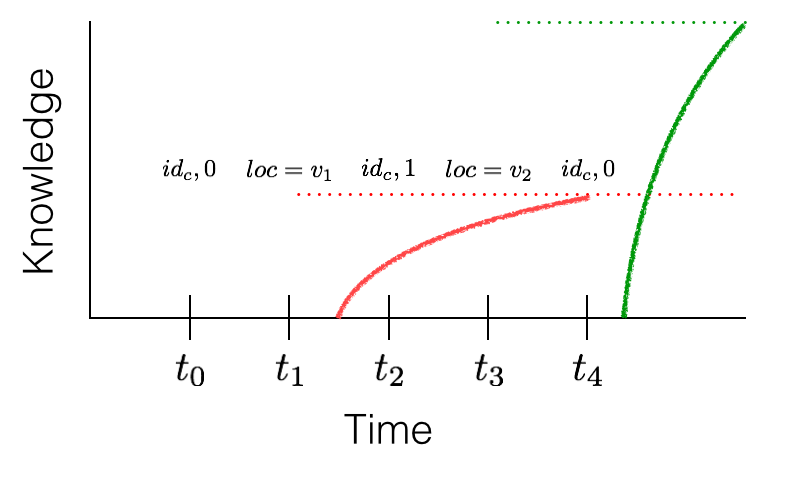
\includegraphics[width=\linewidth]{knowledge-time-graph}
\caption{An illustration of the policy for the location truncation
  app.}
\label{fig:knowledge-time-graph}
\end{figure}

We explain an example statement of this policy in
figure~\ref{fig:knowledge-time-graph}.  At time $t_0$ the user changes
the upper bound on knowledge to be truncated by clicking the checkbox
and button.  At time $t_1$ the location is read, and the upper bound
of knowledge at all future times (illustrated by the dotted red line)
is established to be with truncated granularity because the $Fine$
predicate holds.  The solid red line shows how the observer's
knowledge might actually grow over time, never exceeding the upper
bound.  At time $t_3$, the location is read again, except that as the
user toggled the checkbox, the policy is now more premissive: because
$Fine$ no longer holds, there is no constraint on future knowledge
about the data.  Notably, the formula contains two uses of the
$\talways$ modality.  The first ranges over when data can be
introduced (e.g., times $t_1$ and $t_3$ in the figure), and the second
ranges over when data can be learned (e.g., the solid lines in the
figure).

We can expand the gradual release policies from the previous section
to talk about release policies for dynamic data:

\begin{Definition}[Gradual release for dynamic data]
  A release condition is an LTL formula $R$, and a formula in our
  logic, $K$, parameterized by two values forming an equivalence
  relation.  A set of release conditions $R_i,\rho_i$ can be used to
  define a gradual release policy:
  
%   \begin{displaymath}
%     \begin{array}{l}
%     \forall v_1, (s?v_1@0) \Rightarrow \\
%     ~~ \talways \Big(
%     \bigwedge\limits_{i=1}^n R_i \rightarrow \big( \forall v_2,
%     K_i(v_1,v_2) \rightarrow \tpossible{\prin} (s?v_2@0) \big)
%     \Big) \\
%   \end{array}
%   \end{displaymath}

% \begin{displaymath}
%   \begin{array}{l}
%     \talways Fine \rightarrow \Big(\exists t, v_1. (loc?v_1@t)
%     \rightarrow \\
%     ~~ \forall v_2. \big(truncate(v_1) = truncate(v_2) \rightarrow
%     \talways \tpossible{\prin} loc?v_2@t \big) \Big)
%   \end{array}
% \end{displaymath}
\end{Definition}

\section{Program policies in \hyperltltwo} 

We state program security policies in the logic \hyperltltwo
\cite{Clarkson:2014}.  \hyperltltwo allows quantification over paths,
and atomic predicates that speak about the contents of paths.

\subsection{Definition of traces}

In Hypertemporal logics, traces are regarded by the set of atomic
propositions that are true about them.  In our case, traces are (as in
the ETL section) composed of sequences of timestamped events that
occured in the system, generated by the semantics for a given program.
In other words, the set of (atomic) predictes that holds at a given
time is the set of predicates that holds about a sequence of events
produced by the program from the semantics.

\subsection{Noninterference}

Definition~\ref{defn:noninterference} states our version of
noninterference, for programs that read secret eventful input.  In our
setting, observers reaad events on a subset $\prin$ of channels.
However, while some internal events (such as reads on channels for GUI
inputs) may not be observable they may cause nondeterminism from the
perspective of $\prin$.

Generalized noninterference \cite{} is a security property that allows
nondeterminism in low inputs to the system.  Generalized
noninterference protects secret input events (in our case, reads from
secret channels), typically called \emph{high} input events.  All
other input events are unconstrained, and called \emph{low} events.
This formulation allows us to express noninteference for secret
streams where the policy designates whether or not the current secret
can be released.  It does not, however, allow us allow us express
policies of the form where a portion of the secret is leaked.

We must first define which events are secret.  We define a policy as a
function that takes an event sequence to the set $\{H,L\}$, and tells
us the label of the last event in the sequence:

\begin{displaymath}
  \begin{array}{c}
    policy : \tr \rightarrow \{H,L\}
  \end{array}
\end{displaymath}

As an example, one policy takes an event sequence to $H$ if the last
event is a read from the location channel, and that read has been
proceeded by a value of $0$ on the checkbox channel.  This also allows
us to define policies by an LTL formula $\phi$ on a trace, the policy
would take a trace to $H$ if the last element in the sequence was a
secret and the trace did not satisfy the formula $\phi$, and $L$
otherwise.  Definition two assumes that all inputs from secret
channels are always high, which is expressed by the policy that is $H$
is the last event is an input from a secret, and $L$ otherwise.

\begin{Definition}[Generalized Noninterference]
  A program $e$ satisfies generalized noninterference if, we have
  that:

  \begin{displaymath}
    \begin{array}{l}
      e \models \forall \tr. \forall \tr'. \exists \tr''. \tr =_{H,in}
      \tr'' \land \tr' =_L \tr''
    \end{array}
  \end{displaymath}

  Where the equivalence relations (on traces) $=_{H,in}$ and $=_L$
  compare event sequences after projecting elements by the applicaiton
  of some policy.
\end{Definition}

\begin{Theorem}[GNI implies NI]
  For a particular program e, we have that if:
  \begin{displaymath}
    \begin{array}{c}
      \traces{e} \models GNI
    \end{array}
  \end{displaymath}
  
  Then $e$ satisfies (Definition~\ref{defn:noninterference}), assuming
  the policy maps inputs on secret channels to $H$.
\end{Theorem}

\begin{Proof}
  Assume that $e$ satisfies GNI, we now show that it satisfies
  Definition~\ref{defn:noninterference}.  Consider that it does not.
  This means that there is some $S_1$, $S_2$, and $\tr_1$ such that $e
  \Downarrow S_1 \vdash e \Downarrow \tr_1$ and there is no $\tr_2$
  such that $S_2 \vdash e \Downarrow \tr_2$ and $\tr_2 \equiv_\prin
  \tr_1$.

  Instantiate the formula for GNI with $t = \tr_1$, $t' = \tr_2$, $t''
  = \tr_1$.  The fact that the program satisfies GNI implies that this
  can be done for any $\tr_2$ (because of the universal quantifier for
  $t'$) , and in particular any trace $\tr_2$ such that $S_2 \vdash e
  \Downarrow \tr_2$.  Because GNI implies that $\tr_2 \equiv_\prin
  \tr_1$, we have a contradiction.
\end{Proof}

\paragraph*{``What'' declassification}

\kris{Text out of date}

Let's just assume for simplicity that our programs only deal with an
initial secret, i.e., the program reads its input at time 0 (as its
first reduction).

First, lets talk about ``what'' declassification.  In what
declassification, the observer is never allowed to learn anything
about the secret beyond some equivalence class.

\begin{Definition}[``What'' declassification in HyperLTL]
  \label{defn:hyper-what-declass}
  \begin{displaymath}
    \begin{array}{l}
    \forall p_1, p_2. \forall \pi. \exists \pi'. \\
    ~~ input_0(\pi,p_1) \land input_0(\pi,p_2) \land p_1 \equiv^P p_2
    \rightarrow \\ 
    ~~~~\pi =_L \pi'
    \end{array}
  \end{displaymath}
\end{Definition}

Note that in this formula I used this $\equiv^P$, which is the
equivalence relation up to which the observer is allowed to learn.  An
example would be the parity.  This is a predicate that has to be built
into the logic.  We would have to add atomic predicates that talk
about equality of things in the same fashion that we have to do with
ETL.

\paragraph*{``Where'' declassification}

\kris{Text out of date}

We also have declassification policies that talk about sequences of
events allowing things to be released.  Let's start simple, let's say
that under some condition, the partity is allowed to be released, but
not before then.

Then what we need to say is that for all traces, if the value hasn't
been declassified in both traces, then noninterference should hold.

\begin{Definition}[``Where'' declassification example]
  \label{defn:hyper-noninterference}
  \begin{displaymath}
    \begin{array}{l}
      \forall S_1, S_2. \forall \pi. \exists \pi'. input~\pi,S_1 \land
      input~\pi',S_2 \rightarrow \\
      ~~\talways \big( (\lnot declass~\pi \land \lnot declass~\pi')
      \rightarrow \pi =_L \pi' \big)
    \end{array}
  \end{displaymath}
\end{Definition}

\subsection{Checking symbolic traces for GNI}

Our symbolic executor produces symbolic traces.  These symbolic traces
contain sequences of reads and writes on channels, where the values
written are either primitive values in the underlying logic of the SMT
theory, or are symbolic variables.  A symbolic trace is a sequence of
events of the form $ch?v_s$ or $ch!v_s$ along with a path condition
$\Phi$, where $v_s$ is a symbolic value: either a concrete value (such
as a bit vector) in the logic or a symbolic variable.  While we used
the metavariable \tset to describe the set of traces, we use the
metavariable \tsets to describe a set of symboic traces.

\begin{Definition}[Symbolic trace]
  A symbolic value $v_s$ is either a number or a symbolic variable.

  A symbolic trace is a sequence of the form $ch?v_s$ or $ch?v_s$,
  where $v_s$ is a symbolic value.
    
\end{Definition}

We assume that our symbolic executor produces a finite set of symbolic
traces.  This finite set of traces represents a larger set of actual
executions, because symbolic inputs allow representing multiple
concrete inputs with their abstractions.

For simplicity, assume that the only symbolic inputs in symbolic
traces are secret inputs (for example, assume that all
nondeterministic user inputs will be finite in range and are
concretely specified).  The problem with allowing symbolic GUI inputs
is that it is less obvious how to define the policy function (because
it cannot, for example, simply check an LTL policy, it has to them
form an equation relying on the path condition as well).

Because of this, our policies are specified as functions on traces.
They take trace prefixes to elements of the set $\{H,L\}$, denoting
high or low respectively.  We assume that this function is computable
on traces.  One example function would look at the sequence and see if
the last element of the spinner channel \code{id_s} was $0$ and if so
return $H$ and low otherwise.

Assume the set of symbolic traces is represented by $T =
(\tr_i,\Phi_i)_{i \in [1..n]}$.  Each element of $T$ represents a set
of concrete traces, but some of these sets are empty, because their
path conditions are unsatisfiable.  Consider instead the set $T' =
(\tr_i,\Phi_i)_{i \in [1..k \leq n]}$ which is the same as $T$ except
that we remove all of the unsatisfiable traces from $T$ (to do so we
assert that the path condition is satisfiable to the SMT solver).
(E.g., this would be a \code{filter(is_sat)} in OCaml.)

From $T'$, we form the set of paths $P = T' \times T' \times T'$.
From this set we take all collections of the first two components
($\tr$ and $\tr'$), and for each element $\tr''$ of $T'$ we form the
following equation:

\begin{displaymath}
  \begin{array}{l}
    \forall x_i \in FV(\tr), x_k \in FV(\tr'), \tr =_{H,in} \tr''
    \land \tr' =_L \tr'' \\
    ~~\land \Phi \land \Phi' \land \Phi''
  \end{array}
\end{displaymath}

Together, this set is represented by a conjunction of disjunctions
forming a set of constraints that need to be checked by the SMT
solver.  All in all we denote this formula by $GNI^s(\tsets)$:

\begin{Definition}[Symbolic execution constraint for GNI]
  Applying the transformation, we call this set of constraints
  $GNI^s(\tsets)$.
\end{Definition}

(Note that in the above, care must be taken to hygenically rename
symbolic variables in each of the traces.  I.e., since we are
considering the set $T' \times T' \times T'$, we must properly rename
each of the symbolic variables in the constituent components of the
symbolic traces.  Otherwise we end up with our quantifiers in the
above constraint saying something we don't really mean.)

For each element of $T'$ (the $\tr''$) we ask if this equation is
satisfiable.  If it is, for at least one of the $\tr''$ and every
$\tr$ and $\tr'$, then the program satisfies GNI.  If not, then we get
a counterexample in the form of three traces.  We need one utility
function to relate the concrete semantics to the abstract semantics:

\begin{Definition}[Concrete set of traces from an symbolic set]
  We define the set of traces $\tset = concretize(\tsets)$ to be the
  set of traces such that for each $\tr$, $\tr$ is in $\tset$ if and
  only if instantiating the symbolic variables in the trace with
  concrete values will lead to a satisfiable constraint set.
\end{Definition}

Note that this is a constraint with quantifiers.  I'm not sure how Z3
will handle this right now.

\begin{Theorem}[Soundness of symbolic execution for GNI]
  We have that if:
  
  \begin{displaymath}
    \begin{array}{c}
      \models^{SMT} GNI^s(\tsets)
    \end{array}
  \end{displaymath}
  
  Then the set of traces $\tset = concretize(\tsets)$ satsifies GNI.
  (\kris{This neesds to be fixed, GNI and \hyperltltwo speak about a
    set of infinite traces rather than a set of finite traces.
    Obviously these traces are finite since they were generated by a
    symbolic executor that executes up to some bound.})
\end{Theorem}

\begin{Proof}
  To be completed...
\end{Proof}

\subsection{Optimizing generated formulas}

The formula given above for checking noninterference generates
$O(n^3)$ constraints to be checked by the SMT solver, where $n$ is the
set of symbolic paths produced by the symbolic executor.

One potential optimziation can reduce this to $O(n)$ constraints by
self composing each path with itself, rather than path triples.

Assume that $T$ is the set of symbolic paths generated by the symbolic
executor.  After symbolically executing each path up to some bound, we
take the set of symbolic variables and produce this set of formulas:

\begin{Definition}[Symbolic execution constraint for GNI]
  For each symbolic trace in $\tr,\Phi \in \tsets$, form the following
  constraint:

  \begin{displaymath}
    \begin{array}{c}
      \forall x_i \in FV(\tr), x_k \in FV(\tr'), \tr =_L \tr' \\
      ~~\land \Phi \land \Phi'
    \end{array}
  \end{displaymath}
  
  Where $\tr',\Phi'$ is a hygienically renamed version of $\tr$.
  
  Call this set of constraints $SC(\tsets)$.
\end{Definition}

\begin{Theorem}[$SC(\tsets)$ implies $GNI^s(\tsets)$]
  If:
  
  \begin{displaymath}
    \begin{array}{c}
      \models^{SMT} SC(\tsets)
    \end{array}
  \end{displaymath}
  
  Then:

  \begin{displaymath}
    \begin{array}{c}
      \models^{SMT} GNI^s(\tsets)
    \end{array}
  \end{displaymath}
\end{Theorem}

\begin{Proof}
  To be complted...
\end{Proof}

\section{Enforcing TVETL policies with symbolic execution}
\label{sec:symbolic}

To check the policies discussed in the previous sections, we have
built a symbolic executor which produces sets of program traces and
performs the appropriate checks on traces to ensure that the security
policies are enforced.  We have extended the symdroid \cite{symdroid}
symbolic executor with the necessary GUI elements and model of the
Android system components to implement all of our example apps
disccused in section~\ref{sec:examples} in the Android framework.

Our symbolic executor produces sets of \emph{symbolic} traces that
contain symbolic variables, along with constraints for these
variables, so that a symbolic trace represents a set of concrete
traces.  Using symbolic variables allows us to (e.g.,) make
nondeterministic reductions in input variables with a single trace.
After collecting a set of symbolic traces, we use the set of symbolic
traces to produce proof obligations that must be discharged using a
solver, we use Z3 \cite{z3} and have extended symdroid's interface to
produce proof obligations for our theory.

While the formalism given in section~\ref{sec:formalism} is abstract,
our examples are implemented in Java and link against the Android
framework.  In Android, applications execute inside of a lifecycle
that performs the roles of a state machine to initialize the
application, allowing the application to register callbacks to handle
GUI events and query for the current location and use APIs to access
protected components (such as the phone number).  Symdroid replaces
some of these APIs with custom hooks that allow it to model symbolic
inputs.  As an example, to retrieve the location, an application
interacts with the \code{LocationManager} class and registers a
callback requesting the location.  In symdroid, the callback is
proxied in the symbolic executor so that when it is called it returns
a symbolic variable.

While Android applications are implemented in Java, they actually
share a common structure with the core formalism presented in
section~\ref{sec:formalism}: the main thread is a handler that manages
a message queue implemented in native code by the \code{Looper} class
in Android.  In our symbolic executor, as in the formalism presented
in figure~\ref{fig:formalism}, we nondeterministically explore input
event sequences to cover the input space of the program.

% \begin{figure}[t]
%   \begin{displaymath}
%     \begin{array}{lrcl}
%       \hbox{cst} & \xv & ::= & x n \mid f(\xv_1, \ldots, \xv_i)  \\
%       v
%       \mid x
%       \mid e_1~e_2
%       \mid \sref{e}
%       \mid \sassign{e_1}{e_2}
%       \mid \;\sderef{e} \\
%       && \mid & \scase{e}{\aset{f(x_{i1}, \ldots, x_{ij}) \rightarrow
%           e_i}_{i\in 1..k}} \\
%       && \mid & \sinstall{\sch}{e}
%       \mid \ssend{\sch}{e} \\
%       \hbox{constrs} & f & ::= &
%       \sfmt{none} \mid \sfmt{some} \mid \sunit \mid \cdots \\
%       \hbox{channels} & \sch^{\{i,o\}} & ::= & \sfmt{netin} \mid \sfmt{netout}
%       \mid \cdots \\
% %      \hbox{types} & \typ & ::= & \tint \mid \sch(\typ_1, \ldots, \typ_i) \\ \\
%     \end{array}
%   \end{displaymath}    

%   % \begin{displaymath}
%   %   \begin{array}{ll}
%   %     \loc \in \textit{Locations}
%   %   \end{array}
%   % \end{displaymath}
    
%   \begin{displaymath}
%     \begin{array}{rcll}
%       \Sigma & = & (M, \sigma, H,i) & \hbox{State} \\
%       \evt & : & \sch ? p @ i \mid \sch ! p @ i \mid \tau @ i & \hbox{Message} \\
%       M, t & : & \sch , p ~ \textit{list} & \hbox{Message queue}\\
%       \sigma & : & \loc \partialfun  v & \hbox{Heap} \\
%       H & : & \sch \partialfun \lambda x.e & \hbox{Handler map} \\
%       S & : & \sch \rightarrow i \rightarrow p & \hbox{Secrets}
%     \end{array}
%   \end{displaymath}
%   \caption{Source language syntax and semantic definitions}
%   \label{fig:lang}
% \end{figure}

\subsection{Checking traces with static variables}

Our symbolic traces are simply traces that contain symbolic variables
along with a constraint set that is passed to the solver.  One of the
simplest questions we might ask is whether noninterference holds for
the set of traces.  To check this we will form the following equation:

\begin{displaymath}
  \begin{array}{c}
    NI = \bigwedge\limits_{p_1 , p_2 \in P \times P} p_1
    \restrict_{\prin} = p_2 \restrict_{\prin}
    \wedge ... \wedge p_1^c \wedge p_2^c
  \end{array}
\end{displaymath}
  
Where $p_1\restrict_{\prin}$ is a list of the outputs observable to
$\prin$, and we use $=$ on lists to denote pointwise equality
constraints.

\subsection{Formulating conditions for the SMT solver}

\subsection{Results}

\paragraph*{Runtimes}

We ran symdroid on all of the examples presented in
section~\ref{sec:examples}.  Here are some of the results we got:

\begin{tabular}{ | l || c | c | c | }
  \hline 
  Application & \# of paths & \# of formulas & runtime \\
  \hline
  Contact picker & 1 & 2 & 3 \\
  Bump & 1 & 2 & 3 \\
  Location toggle & 1 & 2 & 3 \\
  Geofencing & 1 & 2 & 3 \\
  Location query & 1 & 2 & 3 \\
  \hline
\end{tabular}

\paragraph*{Examples of interfering programs}

\kris{This figure is wrong, it needs to be updated to hold the actual
  semantics that I worked out in Ott, it's just not copy-pasted there
  yet.}

\subsection{Here's an argument why symbolic execution is sound}

\section{Implement symbolic execution for Android}

Things that need to appear in this section:

\begin{itemize}
\item Overview of symdroid

\item Runtime for symdroid w/ ETL formulas

\item Tricks that we used to get it work

\item Example programs that we actually ran it on, presumably the
  examples from the first section of the work.
\end{itemize}

\section{Related Work}
\label{sec:related-work}

%There have been several efforts to scale up traditional batch based
%security statements (such as noninterference) to an interactive
%setting.  

Our work is most heavily influenced by, and extends (by the theorems
in section~\ref{sec:etl}) the logic of \cite{Balliu:11}.  Our work
differs from that work by presenting an extension of ETL that focuses
on dynamic inputs, and the connection of user input
configurations to release conditions for secret data.  Along with
this, a central goal of our work is to enforce our ETL policies using
symbolic execution.  While \cite{Balliu:11} presents a models
relations for traces, our work focuses on using symbolic traces to
make program checking tractable, presents a core semantics for
reactive programs, and implements this semantics for an implementation
of Android applications.

Bohannon et al.~\cite{Bohannon:09} present \emph{reactive
  noninterference}, which is related to our work in that they focus on
an execution model very similar to ours.  That work states
noninterference for programs that react to events (such as button
clicks in a GUI), with browser-based programs as a primary motivation.
The basic definition of security is essentially the same as that of
\cite{Balliu:11}, but departs in the way the observational equivalence
between traces is defined: leading to notions of termination
sensitivity and different natural statements of security for different
settings.

O'Neill et al.~\cite{O'Neill:06} present information flow for
interactive programs that send and receive on channels and read time
varying data, which we have used to motivate our definition of dynamic
noninterference.  Follow-up work by Clark and Hunt~\cite{Clark:09}
focuses on user strategies, showing that noninterference needs to be
carefully defined based on user input strategies.  The definition of
noninterference they use quantifies over all possible user strategies,
which (as explained in section \ref{sec:tv-ni}) is accounted for by
the definition of trace observation equivalence in the knowledge
modalities.  The work of Rafnsson et al.~\cite{Rafnsson:12} focuses on
extending this work by defining security conditions based on partial
input streams.  This is an orthogonal direction to our work, in the
sense that we consider total streams (i.e., secrets are modeled as
total functions on time) and also programs that are deterministic for
a fixed user input sequence.  We leave it as future work to
investigate how including partial secrets affects the statements of
programs in our logic.

Garg et al.~\cite{Garg:06}: a logic for specifying security policies
of distributed systems.

Chadha et al.~\cite{Lee:09}: using epistemic logic to specify secrecy
policies.

Ahmad and Harper~\cite{Ahmad:13}: under submission, an epistemic logic
formalization of noninterference, including an extension to
declassification.

Sabelfeld and Myers~%\cite{Sabelfeld:04}: \emph{delimited release} (*
MRC: which iirc eventually led to robustness *), which says the
attacker can't exploit declassification to learn more information than
is intended.


Sabelfeld and Sands~%\cite{Sabelfeld:05} present a survey of
declassification that provided axies and terminology for classifying
information release.  Our work is most inspired by Li and
Zdancewic~\cite{Li:05}: \emph{relaxed noninterference}, which
essentially allows declassification through function application.

Halpern and O'Neill~\cite{Halpern:08}: semantic characterizations of
secrecy with epistemic temporal logic.

There is a large body of work that focuses on practical security or
information flow for Android or interactive applications.  Notably,
Enck et al.~\cite{Enck:10} present TaintDroid, a run-time taint
mechanism tracking for Android.  Chong et al.~\cite{Chong:07}: SIF,
information-flow analysis and program splitting for web applications,
including the web-page GUI in the browser. Jia et al.~\cite{Jia:13}
presents run-time enforcement of information flow policies on Android,
backed by a process calculus theory.  To our knowledge, we are the
first to present expressive declassification that is constrained by
user input.

Nanevski et al.~\cite{Nanevski:13}: \emph{Relational Hoare Type
  Theory}, expressing information-flow policies with dependent types.
Aucher et al.~\cite{Aucher:11}: knowledge-based privacy policies that
can change over time. Dimitrova et al.~\cite{Dimitrova:12}:
information-flow policies along with LTL, for specifying when
information must be kept secret and when it may be released. Askarov
and Chong~\cite{Askarov:12}: characterizes leakage of secret
information as change in attacker knowledge. Chong and
Myers~\cite{Chong:04}: declassification policies in a security-typed
language. Roesner et al.~\cite{Roesner:12}: \emph{access control
  gadgets}, which are UI elements that are used to effect access
control policies.  Implemented in Android.

Stateful Declassification Policies for Event-Driven
Programs. Proceedings of the 27th Computer Security Foundations
Symposium (CSF 2014), Vienna, Austria, 19-22 July 2014. \kris{Cite
  this}

\section{Future Work}
\label{sec:future}

\begin{itemize}
  \item Investigate connection between TVETL and Michael / Piotrs work
    on learning values of streams over times
  \item Investigate strategies in inputs ala Rafnsson and how they can
    be encoded in ETL (we deal with synchronous input case here, where
    their semantics can ``get stuck'' with values of bottom)
\end{itemize}

\section{Conclusion}
\label{sec:conclusion}

\bibliographystyle{IEEEtran}
\bibliography{paper}

\appendix 

\section{Translating static ETL to dynamic ETL}
\label{sec:etlb-translation}

\kris{The text in this section is extremely rough.}

Here we present a translation of our ETL formulas to a translation of
those in Balliu et. al \cite{Balliu:11}, which we call \etlb.  The
translation is obtained by observing that our dynamic ETL is a
superset of \etlb, in the sense that we can consider static ETL to be
speaking about the \emph{first} value of a secret stream, where the
program is passed in the secret upon initialization.  To obtain the
computational model of \cite{Balliu:11}, we restrict programs so that
they read in the secret variables as their first input. Furthermore,
since \cite{Balliu:11} do not allow programs to read input, we
disallow any occurences of handlers on input channels.  We are left
with output-only programs that gradually release knowledge about the
secret.  The only element of our computational formalism lacks from
\cite{Balliu:11} is explicit support for loops: these can easily be
encoded by CPS converting a program to use an internal handler that
continually queues a message until the loop condition is false.  While
our logic speaks about any arbitrary set of observable channels to
define observers, \etlb considers all writes to be observable.  In
practical terms, our examples also speak about one observer and we can
use the $\prin$ prefix to translate formulas.  To be precise, we must
also assume that the set of primitives is finite, as in \etlb.

\begin{Definition}[Encoding of \etlb in ETL]
  Assuming $\phi^B$ is a formula is \etlb, we can lift $\phi^B$ to a
  formula in ETL, $\mathcal{F}(\phi^B)$:
  Lifted to our logic using the previous translation we obtain:
  \begin{itemize}
  \item $\mathcal{F}(e_1 = e_2) = \mathcal{F}(e_1) =
    \mathcal{F}(e_2)$, where $\mathcal{F}(e_1)$ is a statement of the
    form $f(s, ..., s)$ representing the equivalent formula.
  \item $\mathcal{F}(init_x(e)) = \exists x . s?x@0 \land x = e$.
  \item $\mathcal{F}(\phi \land \psi) = \mathcal{F}(\phi) \land
    \mathcal{F}(\psi)$.
  \item $\mathcal{F}(\lnot \phi) = \lnot \mathcal{F}(\phi)$.
  \item $\mathcal{F}(\tknows{} \phi) = \tknows{\prin} \mathcal{F}(\phi)$.
  \item $\mathcal{F}(\phi \tuntil \psi) = \mathcal{F}(\phi) \tuntil
    \mathcal{F}(\psi)$.
  \end{itemize}
  Because \etlb assumes a finite domain of primitive values, it
  provides encodings of syntactic sugar for $\forall$, $\exists$,
  $\tpossible{\prin}$, $\tfuture$, $\talways$, and $W$.
\end{Definition}

\subsection{Relation between our AK and \etlb AK}
\label{sec:ak-translation}

Given the previous result, it is unsurprising that the definition of
AK --- used to state noninterference in \cite{Balliu:11} --- can be
lifted to our logic.  Restating here, AK is:

\begin{displaymath}
  \begin{array}{c}
    \talways \forall
    \overrightarrow{v}. \Big(init_{\overrightarrow{l}}(\overrightarrow{v})
    \rightarrow \forall \overrightarrow{u}. L
    \big(init_{\overrightarrow{l}}(\overrightarrow{v}) \land
    init_{\overrightarrow{h}}(\overrightarrow{u}) \big) \Big)
  \end{array}
\end{displaymath}

In \etlb's computation model, the observer is allowed to know the
initial low part of the store.  We do not make the distinction, and
instead use formulas in ETL to protect secret variables, leaving the
others unconstrained .  Removing the low parts of the store, we obtain
the following formula:

\begin{displaymath}
  \begin{array}{c}
    \talways \forall \overrightarrow{u} L
    \big(init_{\overrightarrow{h}}(\overrightarrow{u}) \big)
  \end{array}
\end{displaymath}

Which is translated to the equivalent formula in our ETL:

\begin{displaymath}
  \begin{array}{c}
    \talways \forall \overrightarrow{u}. L_\prin
    \big(\overrightarrow{h}?\overrightarrow{u}@0 \big)
  \end{array}
\end{displaymath}

This is our formula AK shown in section~\ref{sec:encodings}
instantiated with time 0 for $i$ as discussed previously.

\subsection{Relation between static declassification and \etlb AKR}
\label{sec:akr-translation}

Our notion of declassification is similar to that of Balliu et. al
\cite{Balliu:11}: in the case of static data, the formula obtained by
the transformation is equivalent to $AKD$.

\subsection{Equivalence of Noninterference modulo declassification and AKD}

\begin{Theorem}[Equivalence of AKD and Noninterference modulo declassification]
  Assume that $e$ is a program in our formalism containing a single
  secret $\sch$.  Assume that $\rho$ is a release policy. It is true that:
  
  \begin{displaymath}
    \begin{array}{l}
      \forall S_1, S_2, \text{and~} \tr_1, \\
      ~~ S_1 \vdash e \Downarrow \tr_1 \land \equiv^\rho(S_1,S_2) \Rightarrow \exists \tr_2, S_2
      \vdash e \Downarrow \tr_2
      \land \tr_1 \cong_{\prin} \tr_2
    \end{array}
  \end{displaymath}
    
  If and only if: 

  \begin{displaymath}
    \begin{array}{l}
      e \models \talways ~ \Big( \forall v_1, i. ~ \sch ? v_1 @ i \rightarrow \\
      ~~~~~~~~~~ \big( \forall v_2. \rho(v_1) = \rho(v_2) \rightarrow 
      L_\prin(\sch ? v_2 @ i) \big) \Big)
    \end{array}
  \end{displaymath}

\end{Theorem}

\begin{proof}
  To be completed...
\end{proof}

\begin{figure*}[t]
  \small
  \begin{displaymath}
    \begin{array}{c}
      \multicolumn{1}{l}{
        \framebox{$e, \Sigma_1 \sreduce v, \Sigma_2$}
      }
      \\ \\

      \infer[RVal]
      { }
      { v, \Sigma \sreduce v, \Sigma }

      \qquad

      \infer[RApp]
      {
        e_1, \Sigma_1 \sreduce (\lambda x.e_3), \Sigma_2 \\
        e_2, \Sigma_2 \sreduce v_1, \Sigma_3 \\\\
        \aset{x\mapsto v_1}e_3, \Sigma_3 \sreduce v_2, \Sigma_4
      }
      { e_1\;e_2, \Sigma_1 \sreduce v_2, \Sigma_4}

      \qquad

      \infer[RRef]
      {e, \Sigma_1 \sreduce v, \Sigma_2 \\
        \loc \not\in \dom(\Sigma_2.\sigma) \\\\
        \sigma' = \Sigma_2.\sigma[\loc\mapsto v]
      }
      {\sref e, \Sigma \sreduce \loc, \Sigma_2[\sigma \mapsto \sigma']}

      \qquad

      \infer[RAssign]
      {e_1, \Sigma_1 \sreduce \loc, \Sigma_2 \\
        \loc \in \dom(\Sigma_2.\sigma) \\\\
        e_2, \Sigma_2 \sreduce v, \Sigma_3 \\
        \sigma' = \Sigma_2.\sigma[\loc \mapsto v]
      }
      {\sassign {e_1} {e_2}, \Sigma_1 \sreduce
        v, \Sigma_2[\sigma \mapsto \sigma']}

      \\ \\

      \infer[RDeref]
      {e, \Sigma_1 \sreduce \loc, \Sigma_2 \\
       \Sigma_2.\sigma(\loc) = v}
      {\sderef e, \Sigma_1 \sreduce v, \Sigma_2 }

      \qquad

      \infer[RCase]
      {e_1, \Sigma_1 \sreduce f(v_1, \ldots, v_n), \Sigma_2 \\
        \aset{x_i\mapsto v_i}_{i\in 1..n}e_2, \Sigma_2 \sreduce v, \Sigma_3
      }
      {\scase{e_1}{\aset{\ldots, f(x_1, \ldots, x_n) \rightarrow
          e_2, \ldots}}, \Sigma_1 \sreduce v, \Sigma_3}
      \\ \\

      \infer[RInst]
      {
        e_1, \Sigma_1 \sreduce (\lambda x.e_2), \Sigma_2 \\
        H' = \Sigma_2.H[\sch^h \mapsto \lambda x.e_2]
      }
      {
        \sinstall \sch^h {e_1}, \Sigma_1 \sreduce \sunit, \Sigma_2[H
        \mapsto H']
      }

      \qquad

      \infer[RSend]
      { e, \Sigma_1 \sreduce \xv, \Sigma_2 \\
        M' = \Sigma_2.M, (\sch^{\{h,o\}}, \xv)
      }
      { \ssend \sch^{\{h,o\}} e, \Sigma_1 \sreduce \sunit, \Sigma_2[M \mapsto M']}
      \\ \\

      \multicolumn{1}{l}{
        \hbox{\textit{In machine state $\Sigma_1$, expression $e$ reduces to
          value $v$ and updates machine state to $\Sigma_2$.}}
      }

      \\ \\ 

      \multicolumn{1}{l}{
        \framebox{$\Sigma_1 \treduce^{\evt} \Sigma_2$ \hbox{ and } $S
          \judge e \sreduce t$}
      }
      \\ \\

      \infer[THandle]
      { \Sigma_1.M = (\sch^h, \xv), M' \\
        \Sigma_1.H(\sch^h) = \lambda x.e \\\\
        \Sigma' = \Sigma_1[M\mapsto M'] \\
        e \aset{x \mapsto \xv}, \Sigma' \sreduce v', \Sigma_2 \\
      }
      { \Sigma_1 \treduce^{\tau@\Sigma_1.i} \Sigma_2}

      \qquad

      \infer[TOutput]
      { \Sigma.M = (\sch^o,p), M' \\\\
        \Sigma' = \Sigma[M\mapsto M']
      }
      { \Sigma \treduce^{\sch^o!p@\Sigma.i} \tick{\Sigma'}}
      
      \qquad

      \infer[TSecInput]
      { \Sigma' = \Sigma[M \mapsto \Sigma(M) @ (\sch^s, S_{\sch^h}(\Sigma.i))]
      }
      { \Sigma \treduce^{\sch^s?p@\Sigma.i} \tick{\Sigma'} }

      \\ \\ 

      \infer[TInput]
      { \Sigma' = \Sigma[M \mapsto \Sigma(M) @ (\sch^h , p)] \\\\
        \sch^i \in \dom(\Sigma.H)
      }
      { \Sigma \treduce^{\sch^i?p@\Sigma.i} \tick{\Sigma'} }

      \qquad

      % \infer[TLookupSecret]
      % { \Sigma.M = (\sfmt{getsecret},\sch^s,i), M' \\\\
      %   \Sigma' = \Sigma[M\mapsto M' @ (\sch, \Sigma.S(\sch)(\Sigma.i))]
      % }
      % { \Sigma \treduce^{(\sch, \Sigma.S(\sch)(\Sigma.i))} \Sigma'}
      
      % \\ \\ 

      \infer[TProg]
      {
      \Sigma_0 = ([(\code{onCreate},\code{unit})]
                  ,\emptyset
                  ,\aset{\code{onCreate} \mapsto
                          \lambda x . S(e)}
                  ,0)
      \quad x \not\in FV(e) 
        \\\\ 
      \Sigma_i \treduce^{\evt_i} \Sigma_{i+1}
      \quad i \in [0..n]
      }
      { S \judge e { \sreduce \evt_0 \cdot \evt_1 \cdots \evt_n } }

      \\ \\
      \multicolumn{1}{l}{
        \hbox{\textit{Machine state $\Sigma_1$ steps to state $\Sigma_2$ generating
            message $\eta$, and given secret inputs $S$, program $e$
            generates \tr.}}
      }

    \end{array}
  \end{displaymath}
  \caption{Operational semantics}
  \label{fig:symbolic-exec}
\end{figure*}

\begin{figure}[t]
  \begin{displaymath}
    \begin{array}{lrcl}
      \hbox{prims} & \xv & ::= & n \mid f(\xv_1, \ldots, \xv_i)  \\
      \hbox{values} & v & ::= & \xv \mid \loc \mid \lambda x.e \\
      \hbox{operators} & \sfmt{op} & ::= & \code{==} \mid \code{&&}
      \mid \code{||} \mid ... \\
      \hbox{bexprs} & b & ::= &
      p 
      \mid x
      \mid b_1 \sfmt{~op~} b_2 \\
      \hbox{exprs} & e & ::= &
      v
      \mid x
      \mid e_1~e_2
      \mid \sref{e}
      \mid \sassign{e_1}{e_2}
      \mid \;\sderef{e} \\
      && \mid & \scase{e}{\aset{f(x_{i1}, \ldots, x_{ij}) \rightarrow
          e_i}_{i\in 1..k}} \\
      && \mid & \sif{b}{e_1}{e_2} \\
      && \mid & \sinstall{\sch^h}{e}
      \mid \ssend{\sch}{e} \\
      \hbox{constrs} & f & ::= &
      \sfmt{none} \mid \sfmt{some} \mid \sunit \mid \sfmt{true} \mid \cdots \\
      \hbox{channels} & \sch^{\{i,o,h,s\}} & ::= & \sfmt{netin} \mid \sfmt{netout}
      \mid \cdots \\
%      \hbox{types} & \typ & ::= & \tint \mid \sch(\typ_1, \ldots, \typ_i) \\ \\
    \end{array}
  \end{displaymath}    

  \begin{displaymath}
    \begin{array}{lrcl}
      \hbox{symbolic values} & v^s & ::= & p \mid x_s \\
      \hbox{symbolic relations} & R^s & ::= & = \; \mid>\;\mid\;<\;\mid \textrm{mod} \mid + \mid ...  \\
      \hbox{constraints} & c^s & ::= & R^s(v^s_1, ... , v^s_n) \\
      \hbox{constraint set} & \Phi & ::= & c^s_1 \land ... \land c^s_n \\
    \end{array}
  \end{displaymath}    

  % \begin{displaymath}
  %   \begin{array}{ll}
  %     \loc \in \textit{Locations}
  %   \end{array}
  % \end{displaymath}
    
  \begin{displaymath}
    \begin{array}{rcll}
      \Sigma & = & (M, \sigma, H,i) \with \Phi & \hbox{State} \\
      \evt & : & \sch^{\{i,s\}} ? v^s @ i \mid \sch^{\{o\}} ! v^s @ i \mid \tau @ i & \hbox{Message} \\
      M, t & : & \sch , p ~ \textit{list} & \hbox{Message queue}\\
      \sigma & : & \loc \partialfun  v & \hbox{Heap} \\
      H & : & \sch^h \partialfun \lambda x.e & \hbox{Handler map} \\
      S & : & \sch^s \rightarrow i \rightarrow p & \hbox{Secrets}
    \end{array}
  \end{displaymath}
  \caption{Source language syntax and semantic definitions}
  \label{fig:symbolic-lang}
\end{figure}

\end{document}
